\documentclass[a4paper]{ctexart}
\usepackage{xeCJK}
\usepackage{setspace}
\usepackage{fancyhdr}
\usepackage{subfigure}
\usepackage{fontspec,xunicode,xltxtra}
\usepackage{titletoc}
\usepackage[top=29mm,bottom=29mm,left=31.8mm,right=31.8mm]{geometry}
\usepackage{enumerate}
\usepackage{caption}
\usepackage{amsmath,bm}
\usepackage{cite}
\usepackage{enumitem}
\setmainfont{Times New Roman}
\setCJKmainfont[BoldFont={Songti SC Bold}]{SimSun}
\setCJKfamilyfont{heiti}{SimHei}
\renewcommand{\heiti}{\CJKfamily{heiti}\fontspec{Times New Roman}}

\newcommand{\mycaptionfont}{\heiti\zihao{5}}
\captionsetup[figure]{name={\mycaptionfont 图},labelsep=period}
\renewcommand{\captionfont}{\mycaptionfont}
\renewcommand{\captionlabelfont}{\mycaptionfont}

\ctexset {
	section = {
		number = \arabic{section},
		format = \zihao{4}\bfseries,
	},
	subsection = {
		number = \arabic{section}.\arabic{subsection},
		format = \zihao{-4}\bfseries,
	},
	subsubsection = {
		number = \arabic{section}.\arabic{subsection}.\arabic{subsubsection},
		format = \zihao{-4}\bfseries,
	}
}


\setlength\parskip{.5\baselineskip}
\fancypagestyle{plain}{\pagestyle{fancy}}%改变章节首页页眉
\pagestyle{fancy}
\lhead{\kaishu~人工智能课程作业~}
\rhead{\kaishu~1030616134~尹达恒}
\cfoot{\thepage}

\renewcommand{\abstractname}{摘要}
\renewenvironment{abstract}{
	\quotation
	\begin{spacing}{1.2}
		\par\zihao{5}{\bfseries \abstractname:}
	}{\end{spacing}\vskip 2.5ex}

\newcommand{\enabstractname}{Abstract}
\newenvironment{enabstract}{
	\quotation
	\begin{spacing}{1.2}
		\par\zihao{5}{\bfseries \enabstractname:}
	}{\end{spacing}\vskip 2.5ex}

\begin{document}
\begin{center}
	{\zihao{-3}\textbf{人工神经网络理论及应用}}
	
	{\zihao{-4}尹达恒}\\[-1mm]
	
	{\zihao{5}(江南大学物联网工程学院,江苏\quad 无锡)}
\end{center}
\begin{abstract}
	人工神经网络(Artificial neural network,ANN)是现代人工智能研究的重要基石,它克服了过去人工智能中被认为难以解决的一些问题,且随着训练数据量的显著增长以及芯片处理能力的剧增,它在目标检测和计算机视觉、自然语言处理、语音识别和语义分析等领域成效卓然。本文介绍了人工神经网络的基本思想、发展历史和理论基础,综述了目前人工神经网络的主流技术并给出了一些范例,最后探讨了人工神经网络今后的研究方向。
	
	\textbf{关键词:} 回归分析,回归算法,机器学习
\end{abstract}
\begin{center}
	{\zihao{-3}\textbf{The Theory and Application of Artificial Neural Networks}}
	
	{\zihao{-4}YING Da-heng}\\[-1mm]
	
	{\zihao{5}(School of IoT, Jiangnan University, Wuxi Jiangsu, China)}
\end{center}
\begin{enabstract}
	Artificial neural network (ANN) is an important foundation in the field of artificial intelligence. They overcome some problems that were considered difficult to solve for artificial intelligence in the past. And with the significant increase in the amount of training data and the surge in chip processing power, it has achieved outstanding results in the areas of target detection, computer vision, natural language processing, speech recognition and semantic analysis. This paper introduces the basic ideas, development history and theoretical basis of artificial neural network, summarizes the mainstream technology of artificial neural network with some examples, and finally discusses the future research direction of artificial neural network.
	
	\textbf{Keywords:} regression analysis, regression algorithm, machine learning
\end{enabstract}
\begin{spacing}{1.3}
	\zihao{-4}
	\section{简介}
	人工神经网络(Artificial neural network,ANN),又称连接系统(Connectionist system)是受生物神经网络启发而发明的一类信息处理系统。它是从信息处理角度对人脑神经元网络进行抽象而构建出的以有向图为拓扑结构、通过对连续或离散的输入作状态响应而进行信息处理的系统\cite{RN110}。这种信息处理系统集合了多种相互协作的机器学习算法,能够在不对特定任务规则(先验知识)进行编程的情况下从示例中“学习”到抽象的特征表示,并且这些特征表示具有良好的泛化能力\cite{RN114}\cite{RN113}。
	
	人工神经网络的基础是一系列互相连接的单元或节点,称为人工神经元(Artificial neurons)。神经元之间的连接(Connection)能在神经元之间传递一些信号。当一个神经元从神经元连接中得到信号之后,这个神经元能对能对信号进行一些处理并将处理后的信号通过神经元连接再发送给其他的神经元。在人工神经网络的计算过程中,每个神经元都重复着接收信号、处理信号、发送信号的过程,使得信息能在神经网络中传递并变化\cite{RN107}。这种信息的不断传递与变化就是人工神经网络进行信息处理的基本方式。

	对人工神经网络的研究起始于1943年McCulloch和Pitts提出的神经元模型\cite{RN120}。1951年,Donala O.Hebb提出的连接权值强化的Hebb法则\cite{RN124}为构造有学习功能的神经网络模型奠定了基础。然而到了1969年,Minsky和Papert经过多年研究,指出当时的单层神经网络只能应用于简单的线性问题,而不能有效构建多层网络\cite{RN126},由此开始了神经网络的第一个低谷期。直到1986年,Rumehart和Hinton等人提出了用于训练多层神经网络的反向传播算法\cite{RN127},解决了原来一些单层神经网络所不能解决的问题,由此掀起了第二次神经网络研究热潮。但传统的反向传播网络在增加深度时会遇到局部最优、过拟合及梯度扩散等问题,再加之20世纪90年代支持向量机\cite{RN128}等一系列经典的浅层机器学习模型的提出,使得神经网络模型再次陷入低潮。2006年,Hinton等人在《Science》上发文指出\cite{RN129}:(1)多隐层的人工神经网络具有优异的特征学习能力;(2)可通过“逐层预训练”(layer-wise pre-training)来有效克服深层神经网络在训练上的困难,从此引出了深度学习(Deep Learning)的研究,同时也掀起了人工神经网络研究的又一热潮\cite{RN112}。时至今日,随着计算机硬件处理能力的不断提高和神经网络训练数据量的不断增长,人工神经网络及其衍生出的各类深度学习模型正在越来越多的领域取得卓越成效。
	
	本文将首先介绍人工神经网络的基本理论,随后从模型入手介绍一些主流的人工神经网络理论以及一些范例,并在此基础上对当今广泛使用的一些神经网络模型进行综述,最后简要探讨人工神经网络未来的发展方向。

	\section{人工神经网络的基本理论}
	\subsection{人工神经元}\label{sec:人工神经元}
	人工神经元(Artificial Neuron)是人工神经网络的基本处理单元,是神经网络中最基本的组成部分。在生物神经网络中,每个神经元都与其他神经元相连,当神经元被激活(activate)时,就会向相连的神经元发送化学物质改变这些神经元内的电位;如果某神经元的电位超过一定阈值(threshold),那么它就会被激活,进而向其他神经元发送化学物质\cite{RN90}。1943年,McCulloch和Pitts对神经元的活动进行了一定程度的抽象,提出了人工神经元的基本模型\cite{RN120},称为“MP神经元模型”。MP神经元模型是一个多自变量单因变量的函数,包含输入、偏置、激活三个部分,其结构模型如图\ref{figure:neuron}所示。
	\begin{figure}[htbp]
		\centering
		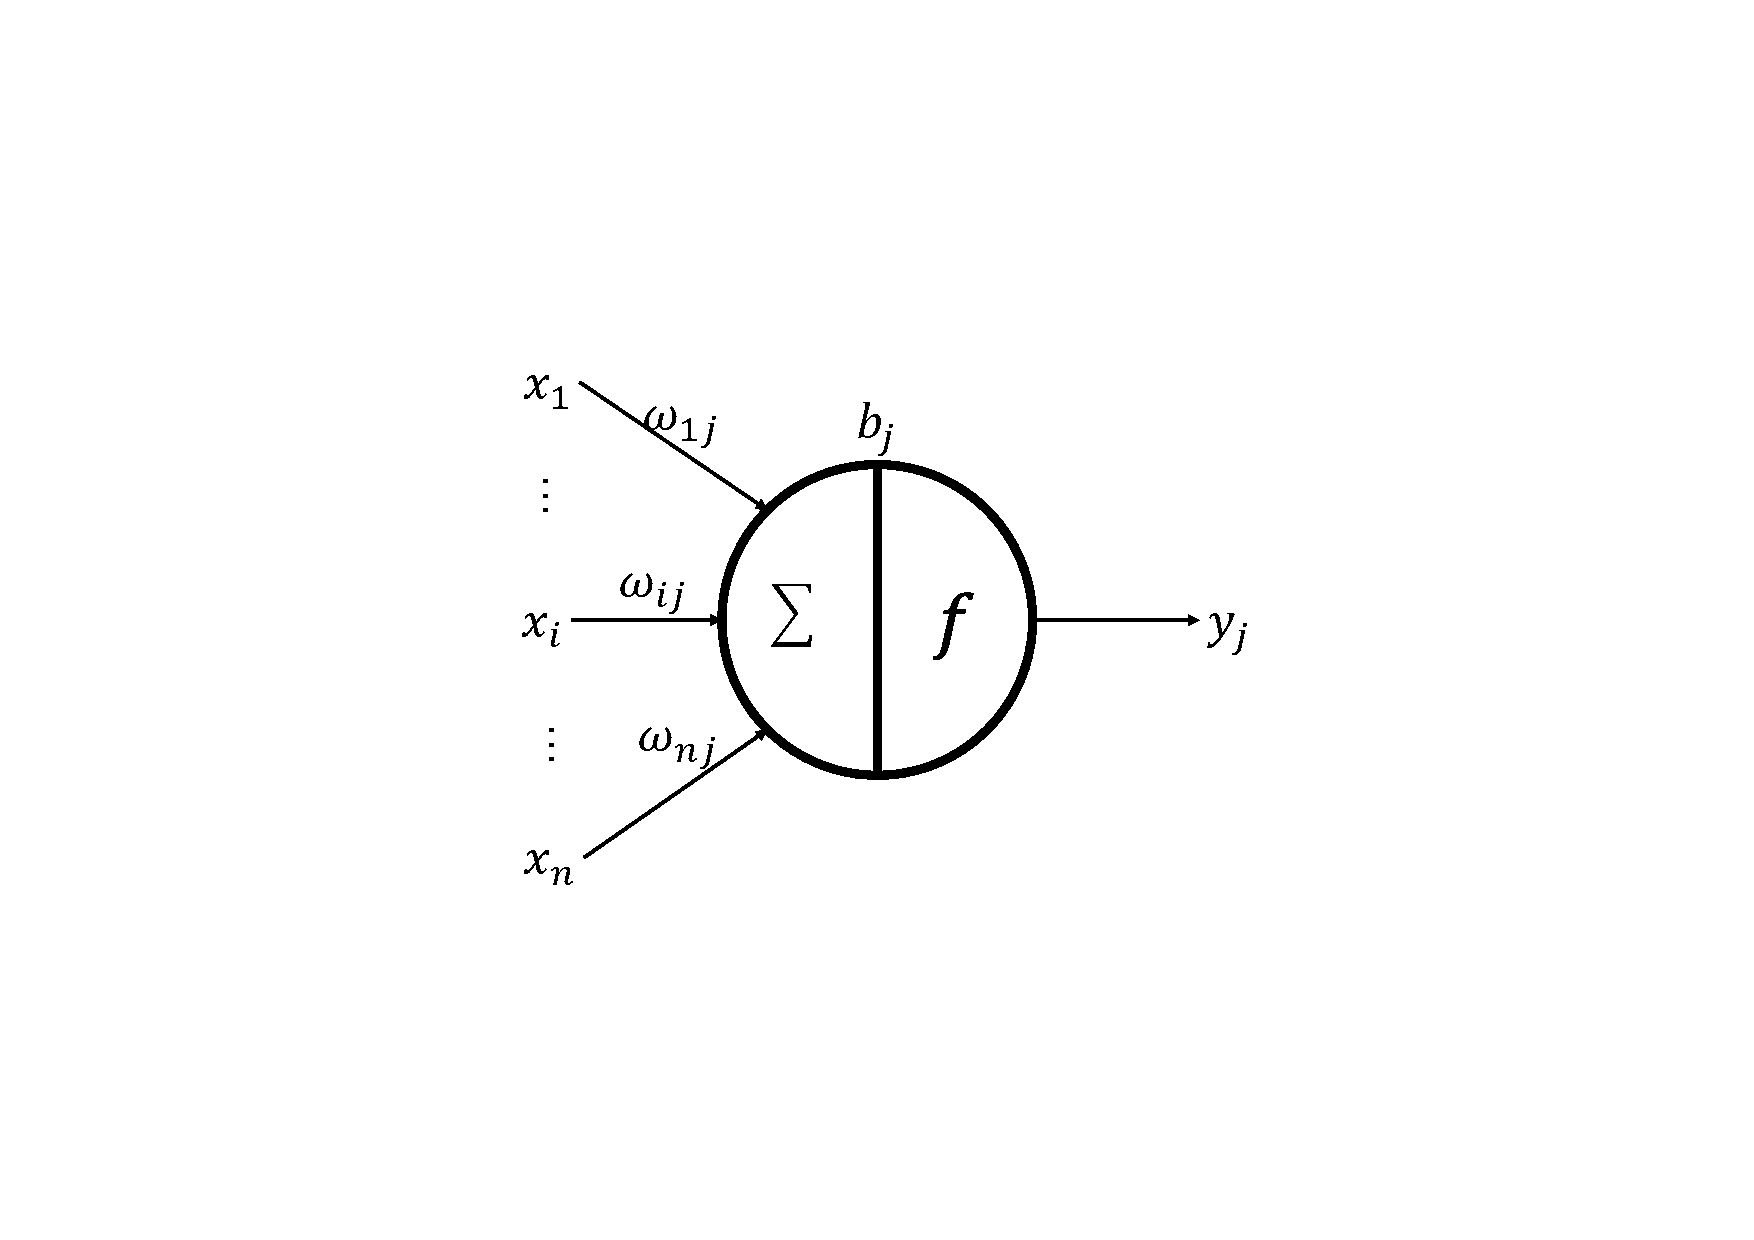
\includegraphics[width=0.6\textwidth, keepaspectratio]{figure/neuron.pdf}\\
		\caption{人工神经元结构图}\label{figure:neuron}


		%TODO:图中没有标出输入、偏置、激活三个部分


	\end{figure}\newline
	其中$x_i$表示输入信号,$n$表示输入神经元$j$的信号个数,$\omega_{ij}$表示输入信号$x_i$与神经元$j$之间连接的权值,$b_j$表示神经元$j$内部的偏置(bias),$y_j$为神经元$j$的输出。在神经元$j$中,输入与输出之间的关系可以用如下公式表示:
	\begin{equation}
		y_j=f\left(b_j+\sum_{i=1}^n\omega_{ij}x_i\right)
	\end{equation}
	其中$f(\cdot)$为激活函数(activate function),它的形式多种多样。若将$b_j$视为一个恒为1的输入$x_0$通过一个$\omega_{0j}=b_j$的权值与神经元相连,则输入与输出关系表达式可以简化为:
	\begin{equation}
		y_j=f\left(\sum_{i=0}^n\omega_{ij}x_i\right)\quad(x_0=1,\omega_{0j}=b_j)
	\end{equation}
	进一步用向量形式表示为:
	\begin{equation}
		\begin{split}
			y_j&=f\left(\bm{\omega}^T\bm{x}\right)\\
			\bm{\omega}&=\left[b_j,\omega_{1j},\dots,\omega_{ij},\dots,\omega_{nj}\right]^T\\
			\bm{x}&=\left[1,x_1,\dots,x_i,\dots,x_n\right]^T
		\end{split}
	\end{equation}
	在人工神经元连接而成的神经网络中,特征并非集中表征于某个函数或变量,而是分散在各个神经元连接的权值中,这种表征方式被称为分布式表征 (distributed representation)\cite{RN123}。和传统的局部表征 (localized representation)相比,分布式表征对特征存储效率较高。线性增加的神经元数目可以表达指数级增加的大量不同概念。这使得类似于神经网络的分布式表征系统大都具有较高的适应性。除此之外,分布式表征的另一个优点是,即使局部出现硬件故障,信息的表达也不会受到根本性的破坏。这使得神经网络对于样本中出现的错误具有较高的容错性。

	但是,单有人工神经元组成的神经网络是不能自行改变神经网络中的连接权值的,要想使得人工神经网络具有“学习”能力,调节人工神经元连接权值的算法必不可少。对人工神经网络权值进行调节的算法多种多样,主要分为两大类:监督学习(Supervised Learning)与无监督学习(Unsupervised Learning)。

	\subsection{监督学习的基础——Delta规则}
	Delta规则(Delta rule)又称Widrow-Hoff规则(Widrow-Hoff rule)\cite{RN125},是一种简单的有导师学习算法。该算法根据神经元的实际输出与期望输出差别来调整连接权,其数学表示如下:
	\begin{equation}
		\omega_{ij}(t+1)=\omega_{ij}(t)+\alpha(y_i(t)-\hat{y_i}(t))x_j(t)
	\end{equation}
	其中$\omega_{ij}(t)$表示计算第$t$个样本时神经元$j$到神经元$i$的连接权值,$y_i(t)$表示神经元$i$期望输出,$\hat{y_i}(t)$表示神经元$i$的实际输出,$x_j(t)$表示神经元$j$的状态,若神经元j处于激活态则$x_j(t)$为1,若处于抑制状态则$x_j(t)$为0或-1(根据激活函数而定);$\alpha$是表示学习速度的常数,称为学习率(Learning Rate)。假设$x_j(t)$为1,若$\hat{y_i}(t)>y_i(t)$,那么$\omega_{ij}$将增大,反之$\omega_{ij}$将变小。

	简言之,Delta规则就是:若神经元实际输出比期望输出大,则减小所有输入为正的连接的权重,增大所有输入为负的连接的权重,从而减小神经元实际输出。反之,若神经元实际输出比期望输出小,则增大所有输入为正的连接的权重,减小所有输入为负的连接的权重,从而增大神经元实际输出。这个增大或减小的幅度由学习率$\alpha$和神经元实际输出与期望输出的差距共同决定。

	\subsection{无监督学习的基础——赫布理论}
	赫布理论(Hebbian theory)又称细胞结集理论(cell assembly theory)是一个神经科学理论,解释了在学习的过程中脑中的神经元所发生的变化。赫布理论描述了突触可塑性的基本原理,即突触前神经元向突触后神经元的持续重复的刺激,可以导致突触传递效能的增加\cite{RN124}。赫布理论可以用于解释“联合学习”(associative learning),在这种学习中,由对神经元的重复刺激,使得神经元之间的突触强度增加。这样的学习方法被称为赫布型学习(Hebbian learning),是最古老的也是最简单的神经元学习规则。赫布理论也由此成为了非监督学习的生物学基础。

	描述赫布学习规则的公式非常简洁:
	\begin{equation}
		\omega_{ij}(t+1)=\omega_{ij}(t)+\alpha y_i(t)y_j(t)
	\end{equation}
	其中$\omega_{ij}(t)$表示计算第$t$个样本时神经元$j$到神经元$i$的连接权值,$y_i(t)$与$y_j(t)$表示计算第$t$个样本时神经元$i$和神经元$j$的输出,输出为正表示激活,输出为负表示抑制;$\alpha$是表示学习速度的常数。若$y_i$与$y_j$同时被激活,即$y_i$与$y_j$同时为正,那么$\omega_{ij}$将增大,表示神经元之间的突触强度增加。若$y_i$被激活,而$y_j$处于抑制状态,即$y_i$为正$y_j$为负,那么$\omega_{ij}$将变小,表示神经元之间的突触强度减小。

	\section{多层感知机}\label{sec:多层感知机}
	多层感知机(Multilayer Perceptron,MLP)是一种由人工神经元组成网络结构,由输入层、隐藏层和输出层构成。多层感知机每一层都包含一个或多个神经元,各层的神经元都以上一层的输出作为输入,并将该层的输出传递到下一层的输入中\cite{RN121}。例如,一个典型的含有两个隐藏层的的多层感知机结构如图\ref{figure:network}。
	\begin{figure}[htbp]
		\centering
		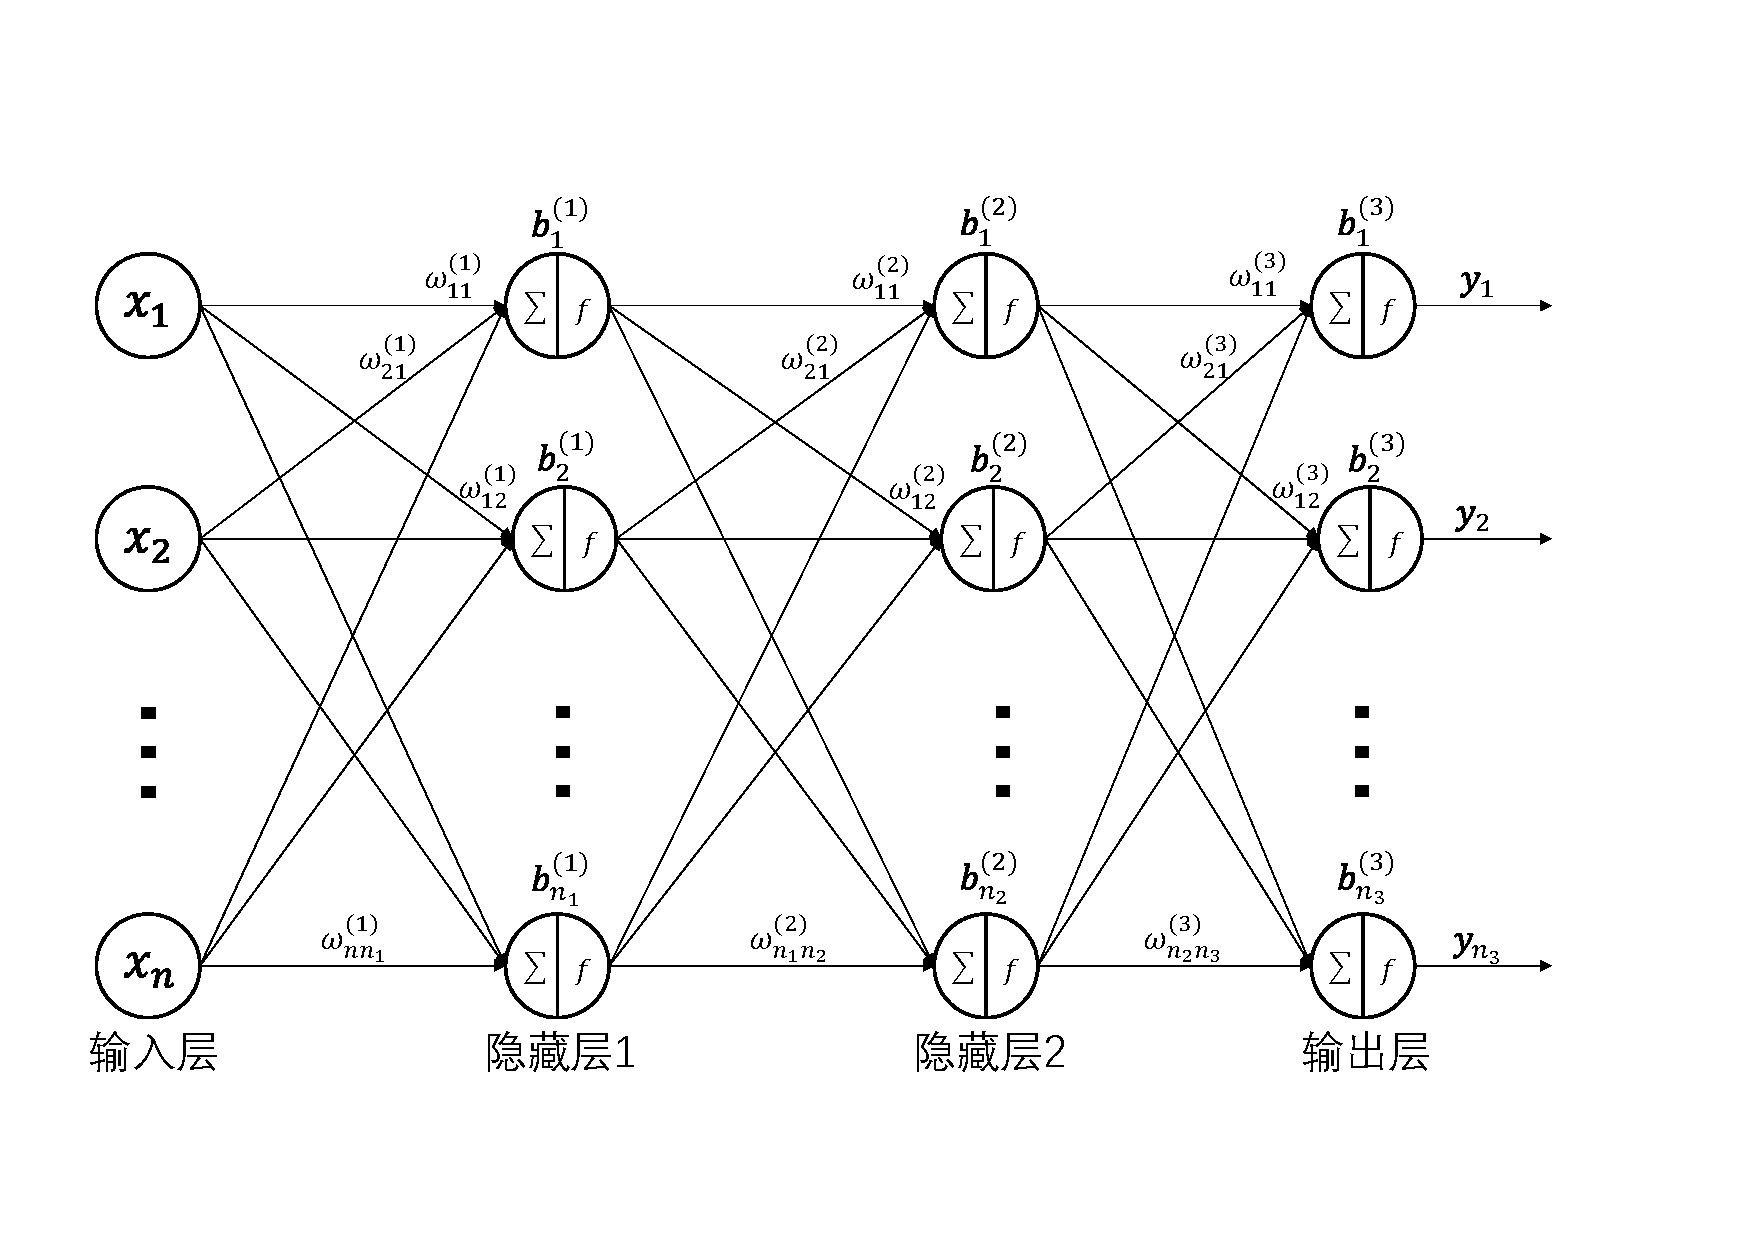
\includegraphics[width=0.9\textwidth, keepaspectratio]{figure/network.pdf}\\
		\caption{多层感知机结构图}\label{figure:network}
	\end{figure}\newline
	其中$n$表示输入层的变量个数,$x_i$表示输入层各变量的值,$n_l$表示第$l$层的神经元个数,$\omega_{ij}^{(l)}$表示第$(l-1)$层的第$i$个神经元和第$l$层的第$j$个神经元之间的连接权值,$y_i$表示输出层各神经元的输出值,通常也作为整个多层感知机的输出。如果以$y_j^{(l)}$表示隐藏层$l$中的第$j$个神经元的输出,且令输出层为第$L$层,则多层感知机的输出$y_j$可以由如下递推公式给出:
	\begin{equation}\label{eq:多层感知机数字形式}
		\begin{aligned}
				y_j&=y_j^{(L)}&(1\leq j\leq n_L)\\
				y_j^{(l)}&=f\left(b_j^{(l)}+\sum_{i=1}^{n_{l-1}}\omega_{ij}^{(l)}y_i^{(l-1)}\right)&(2\leq l\leq L,1\leq j\leq n_l)\\
				y_j^{(1)}&=f\left(b_j^{(1)}+\sum_{i=1}^n\omega_{ij}^{(1)}x_i\right)&(1\leq j\leq n)\\
		\end{aligned}
	\end{equation}
	与\ref{sec:人工神经元}节类似,若将$b_j^{(l)}$视为一个恒为1的输入$y_0^{(l-1)}$通过一个$\omega_{0j}^{(l)}=b_j^{(l)}$的权值与神经元相连,并且将输入层看作第$l=0$层,则递推公式(\ref{eq:多层感知机数字形式})可化为向量形式:
	\begin{equation}\label{eq:前向传播}
		\begin{aligned}
			y_j^{(l)}&=f\left((\bm{\omega}_{j}^{(l)})^T\bm{y}^{(l-1)}\right)&(1\leq j\leq n_l,1\leq l\leq L)\\
			\bm{\omega}_{j}^{(l)}&=\left[b_j^{(l)},\omega_{1j}^{(l)},\dots,\omega_{ij}^{(l)},\dots,\omega_{n_{l-1}j}^{(l)}\right]^T&(1\leq j\leq n_l,1\leq l\leq L)\\
			\bm{y}^{(l)}&=\left[1,y_1^{(l)},\dots,y_i^{(l)},\dots,y_{n_l}^{(l)}\right]^T&(1\leq l\leq L)\\
			\bm{y}^{(0)}&=\left[1,x_1,\dots,x_i,\dots,x_n\right]^T
		\end{aligned}
	\end{equation}
	对于一个多层感知机,在已知输入和各层神经元连接权值的情况下,通过递推公式(\ref{eq:前向传播}),可以从$l=0$开始逐层计算神经元的输出,直到最后得到多层感知机输出层的的输出值$\bm{y}^{(L)}$,这个过程也被称为前向传播(forward propagation)\cite{RN119}。更进一步,若将层与层之间的权值$\bm{\omega}_{j}^{(l)}$用权值矩阵$\bm{W}$的形式表示,则递推公式(\ref{eq:前向传播})可化为矩阵形式:
	\begin{equation}\label{eq:前向传播-矩阵形式}
		\begin{aligned}
			\bm{y}^{(l)}&=f\left(\bm{W}^{(l)}\bm{y}^{(l-1)}\right)&(1\leq l\leq L)\\
			\bm{W}^{(l)}&=
			\begin{bmatrix}
				b_1^{(l)}&\omega_{11}^{(l)}&\dots&\omega_{i1}^{(l)}&\dots&\omega_{n_{l-1}1}^{(l)}\\
				\vdots&\vdots&\ddots&\vdots&\ddots&\vdots\\
				b_j^{(l)}&\omega_{1j}^{(l)}&\dots&\omega_{ij}^{(l)}&\dots&\omega_{n_{l-1}j}^{(l)}\\
				\vdots&\vdots&\ddots&\vdots&\ddots&\vdots\\
				b_{n_l}^{(l)}&\omega_{1n_l}^{(l)}&\dots&\omega_{in_l}^{(l)}&\dots&\omega_{n_{l-1}n_{l}}^{(l)}\\
			\end{bmatrix}&(1\leq l\leq L)\\
			\bm{y}^{(0)}&=\left[1,x_1,\dots,x_i,\dots,x_n\right]^T
		\end{aligned}
	\end{equation}
	递推公式(\ref{eq:前向传播-矩阵形式})即多层感知机前向传播公式的矩阵形式。

	多层感知机是神经网络最基本、使用最广泛的形式。对于一系列给定输入$\bm{x}$和对应的输出$\bm{y}$,多层感知机可以通过改变各层的连接权值,使得对于每个给定的输入$\bm{x}$,多层感知机给出输出向量$\hat{\bm{y}}$和给定输出$\bm{y}$尽可能的逼近(approximate)。George Cybenko曾从数学上证明:包含一个及以上隐藏层的神经网络可以被用来按照任意给定的精度来逼近任何连续函数,且近似精度随隐藏层神经元个数的增加而上升\cite{RN122}。这个定理表明多层感知机是一种具有普适性的函数拟合器,这也是众多深度学习算法有效性的基础。

	图\ref{figure:MLP1}和图\ref{figure:MLP2}展示了8个输入层有两个神经元,输出层有一个神经元的多层感知机的输入和输出关系。这8个多层感知机的权值矩阵均为随机生成的在0-1之间的浮点数,各层激活函数均为ReLU函数。图\ref{figure:MLP1}中所示的4个多层感知机隐藏层由20个神经元组成,而图\ref{figure:MLP1}中所示的4个多层感知机隐藏层由200个神经元组成。由图中我们可以看出,增加了隐藏层的神经元个数后,多层感知机的输出变得更加“灵活”,这也印证了George Cybenko所证明的神经网络的普适性定理。

	\begin{figure}[htbp]
		\begin{minipage}[t]{0.5\textwidth}
			\centering
			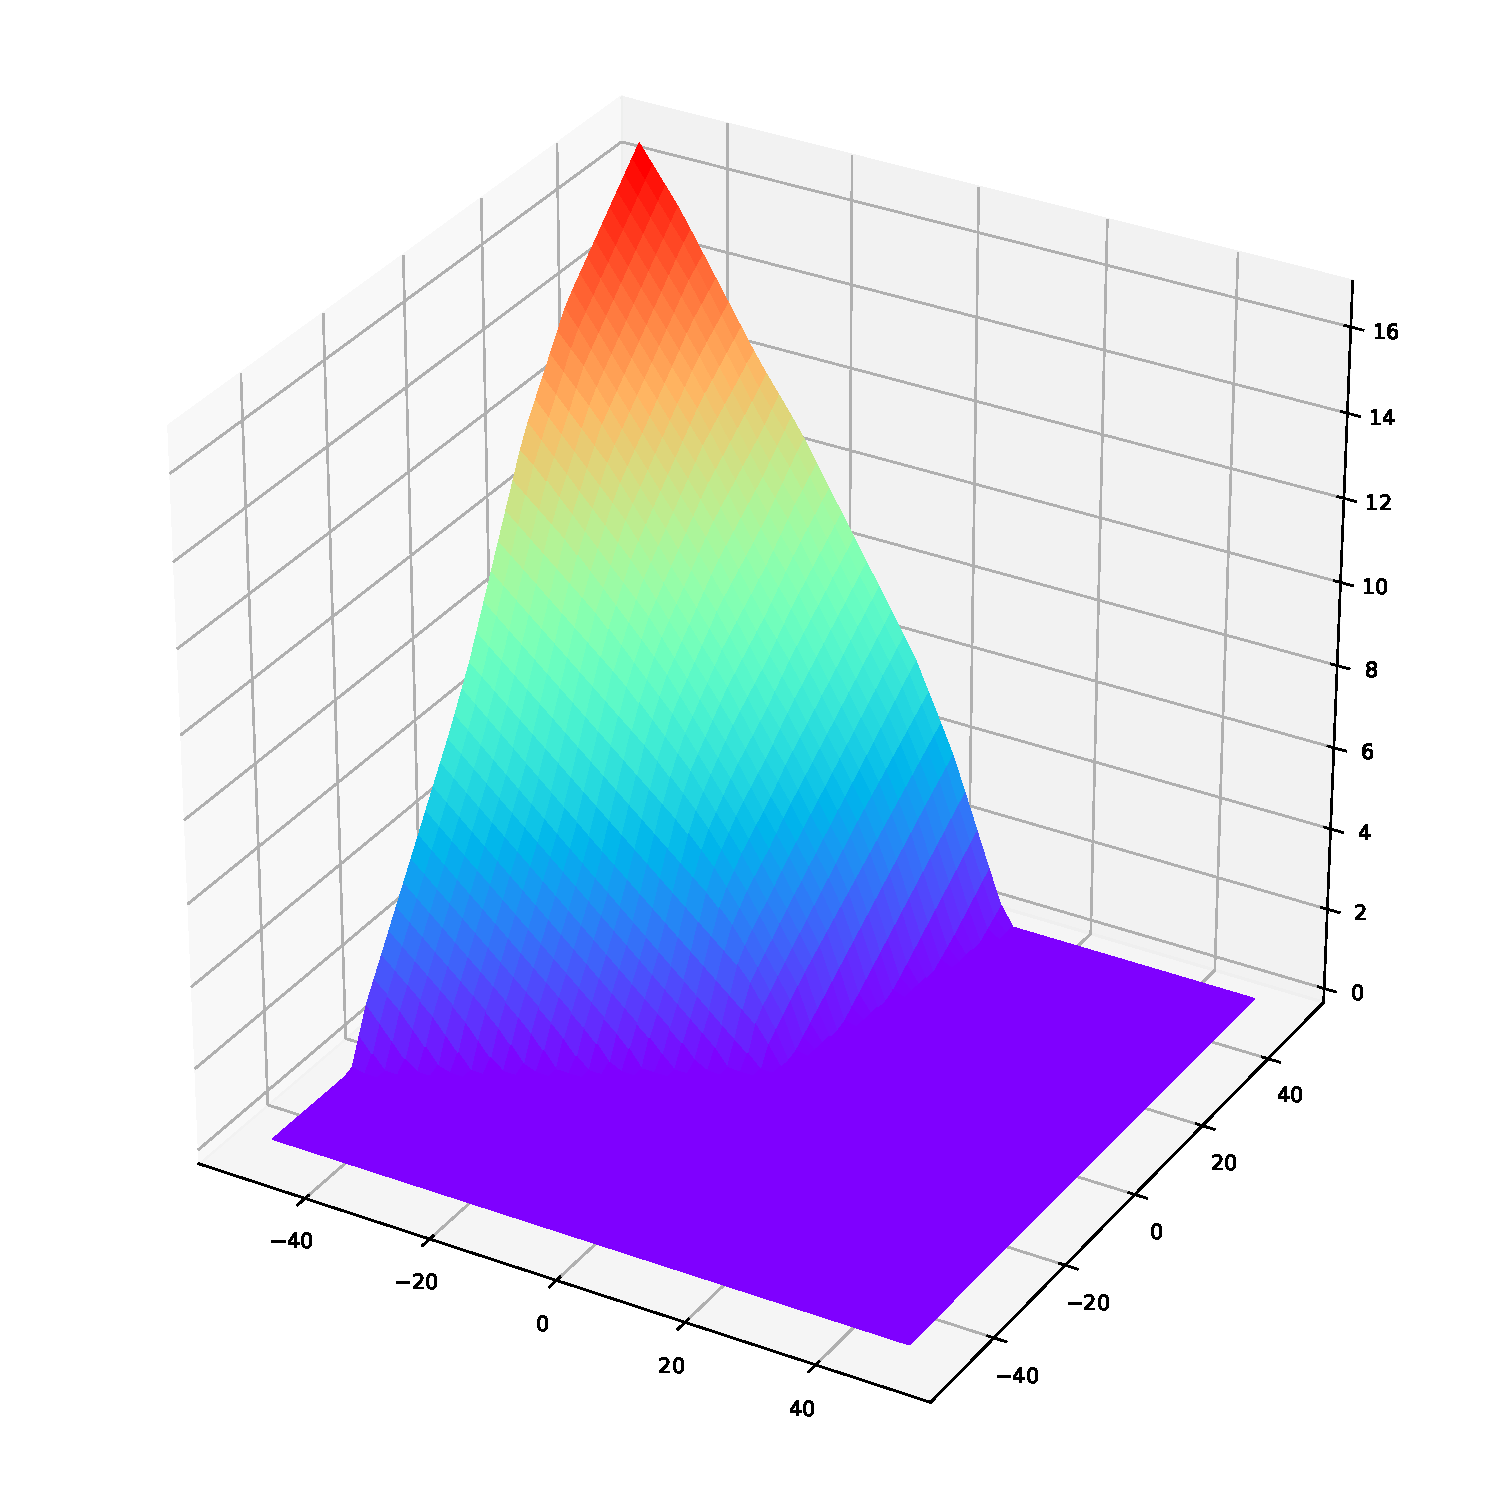
\includegraphics[width=\textwidth, keepaspectratio]{figure/MLP1.pdf}\\
		\caption{隐藏层20神经元的多层感知机}\label{figure:MLP1}
		\end{minipage}%
		\hfill
		\begin{minipage}[t]{0.5\textwidth}
			\centering
			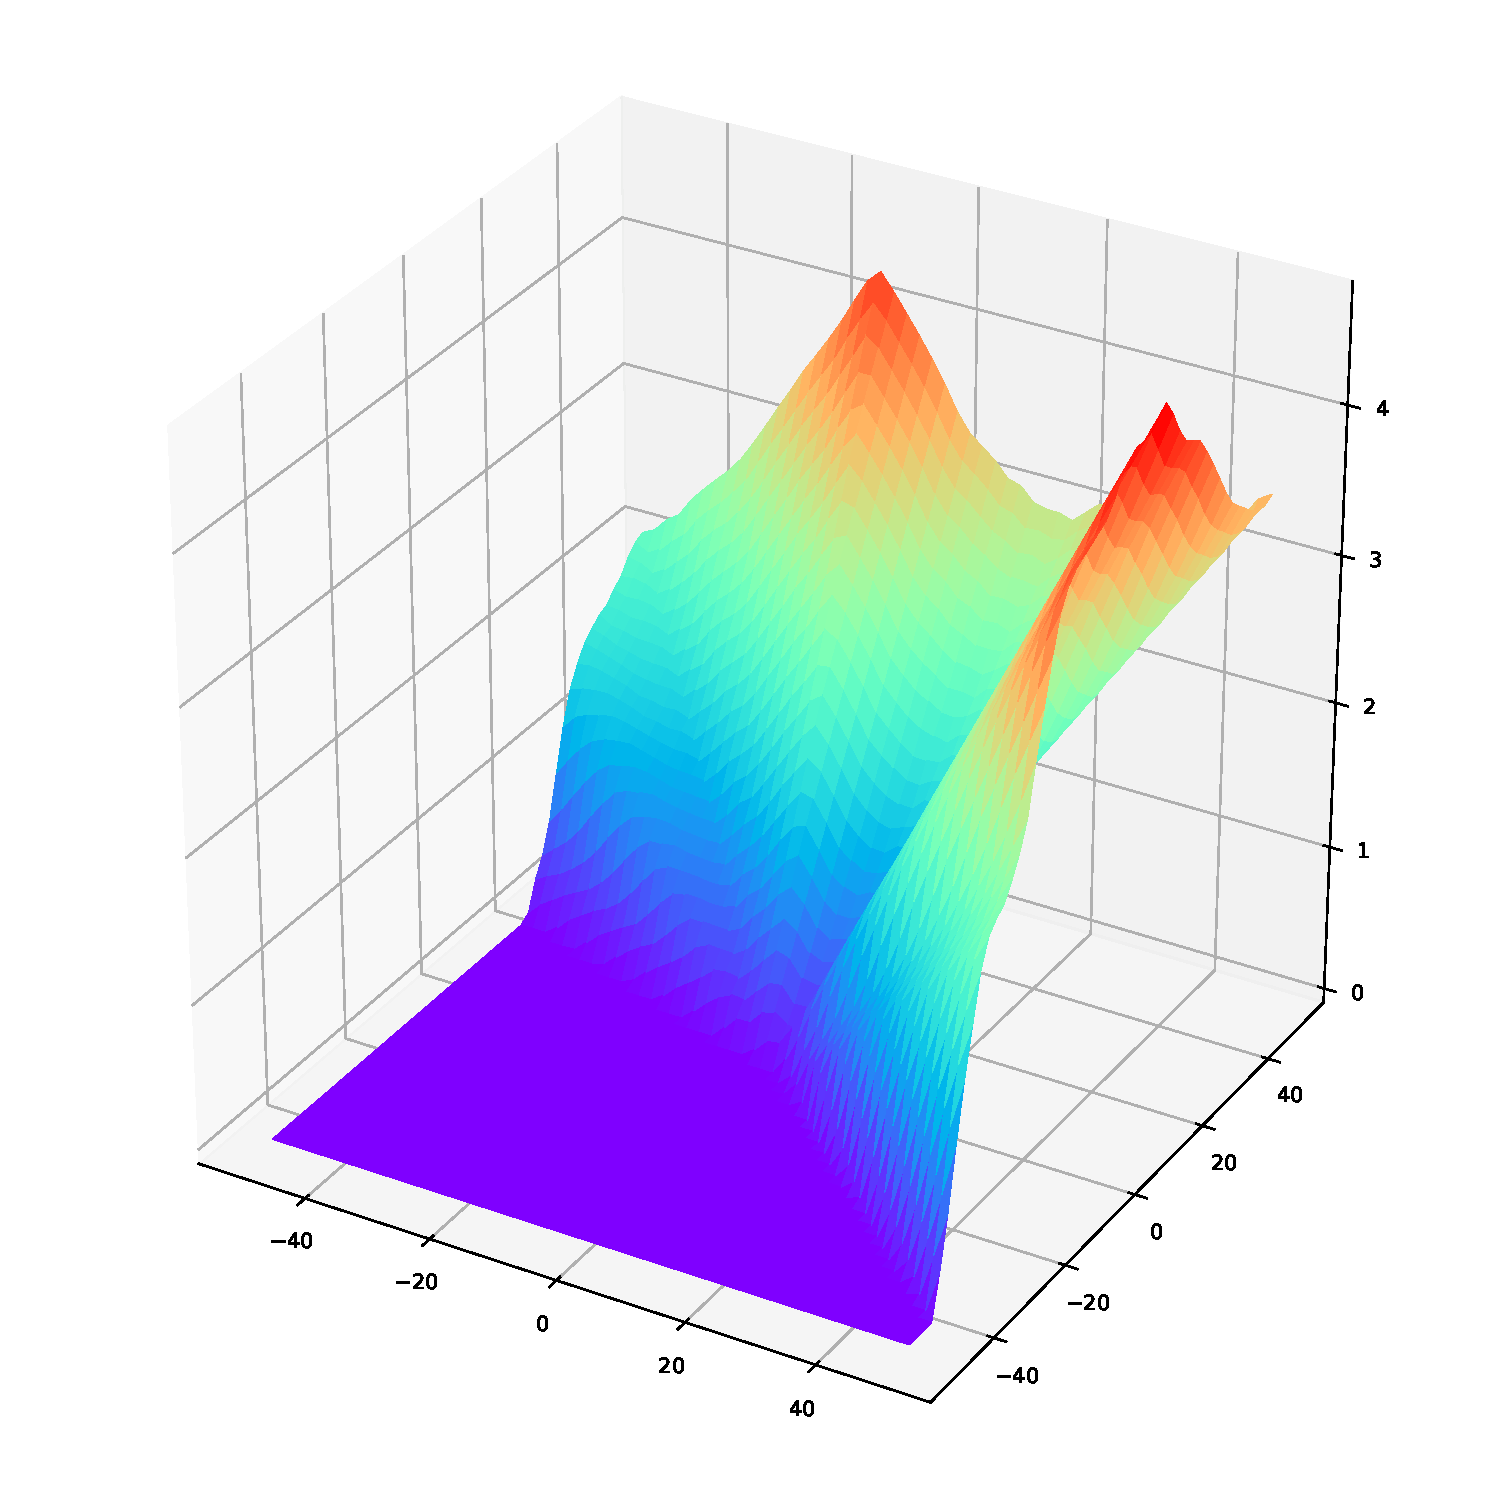
\includegraphics[width=\textwidth, keepaspectratio]{figure/MLP2.pdf}\\
		\caption{隐藏层200神经元的多层感知机}\label{figure:MLP2}
		\end{minipage}
	\end{figure}

	\section{反向传播}
	反向传播(Back propagation)是Rumehart和Hinton等人于1986年提出的用于训练多层神经网络的算法\cite{RN127},其本质类似Delta规则,也是一种按照输出误差对权值进行迭代调整的算法。进行反向传播的方法是梯度下降(Gradient Descent),即在每次迭代过程中,对于网络中的每个权值,都按照它相对于误差的梯度方向进行调整,从而递归性地逼近具有最小误差的模型。在一个多层感知机中,梯度下降有如下公式:
	\begin{equation}\label{eq:权值更新公式}
		\omega_{ij}^{(l)*}=\omega_{ij}^{(l)}-\alpha\frac{\partial E}{\partial\omega_{ij}^{(l)}}
		\quad
		(1\leq l\leq L)
	\end{equation}
	其中,$\omega_{ij}^{(l)}$表示网络中的某个权值,$\omega_{ij}^{(l)*}$表示一次迭代后的权值,$E$表示网络的误差,$\alpha$表示学习率。反向传播的关键是求出权值的梯度$\frac{\partial E}{\partial\omega_{ij}^{(l)}}$。首先考察最后一层的情况,若已知误差$E$与输出层输出值$\bm{y}^{(L)}$之间的函数关系式$E=E(\bm{y}^{(L)})$,即损失函数(Loss Function),则可以由链式法则求得最后一层权值相对于误差的梯度:
	\begin{equation}\label{eq:反向传播-最后一层}
		\begin{split}
			\frac{\partial E}{\partial\omega_{ij}^{(L)}}&=\frac{\partial E}{\partial y_j^{(L)}}\frac{\partial y_j^{(L)}}{\partial\omega_{ij}^{(L)}}\\
			&=\frac{\partial E}{\partial y_j^{(L)}}\frac{\partial f\left((\bm{\omega}_{j}^{(L)})^T\bm{y}^{(L-1)}\right)}{\partial(\bm{\omega}_{j}^{(L)})^T\bm{y}^{(L-1)}}\frac{\partial (\bm{\omega}_{j}^{(L)})^T\bm{y}^{(L-1)}}{\partial\omega_{ij}^{(L)}}\\
			&=\frac{\partial E}{\partial y_j^{(L)}}f'\left((\bm{\omega}_{j}^{(L)})^T\bm{y}^{(L-1)}\right)y_i^{(L-1)}
		\end{split}
	\end{equation}
	若令$t_j^{(l)}=(\bm{\omega}_{j}^{(l)})^T\bm{y}^{(l-1)}$表示第$l$层第$j$个神经元激活前的值,其中$1\leq l\leq L$,则公式(\ref{eq:反向传播-最后一层})可以简写为:
	\begin{equation}
		\frac{\partial E}{\partial\omega_{ij}^{(L)}}=\frac{\partial E}{\partial t_j^{(L)}}\frac{\partial t_j^{(L)}}{\partial\omega_{ij}^{(L)}}=\frac{\partial E}{\partial y_j^{(L)}}f'\left(t_j^{(L)}\right)y_i^{(L-1)}
	\end{equation}
	类似的,对于网络中的每一个连接的权值,可以得到:
	\begin{equation}\label{eq:每一层权值误差简化形式}
			\frac{\partial E}{\partial\omega_{ij}^{(l)}}=\frac{\partial E}{\partial t_j^{(l)}}\frac{\partial t_j^{(l)}}{\partial\omega_{ij}^{(l)}}=\frac{\partial E}{\partial t_j^{(l)}}y_i^{(l-1)}
			\quad
			(1\leq l\leq L)
	\end{equation}
	公式(\ref{eq:每一层权值误差简化形式})表明,连接权值误差的梯度可以表示为神经元激活前的值相对于误差的偏导与该神经元所连接的前一个神经元值的积,其中,神经元激活前的值相对于误差的偏导$\frac{\partial E}{\partial t_j^{(l)}}$又被称为误差信号\cite{RN130}\cite{RN131},用$E_j^{(l)}$表示。因此连接权值误差的梯度表达式(\ref{eq:每一层权值误差简化形式})可以进一步简化为:
	\begin{equation}\label{eq:误差计算}
		\frac{\partial E}{\partial\omega_{ij}^{(l)}}=E_j^{(l)}y_i^{(l-1)}
		\quad
		(1\leq l\leq L)
	\end{equation}
	当已知第$l+1$层的误差信号$E_j^{(l+1)}$时,由链式法则可以求得第$l$层$(1\leq l\leq L-1)$的误差信号$E_i^{(l)}$为:
	\begin{equation}\label{eq:误差传播}
		\begin{split}
			E_i^{(l)}&=\frac{\partial E}{\partial t_i^{(l)}}\\
			&=\frac{\partial E}{\partial y_i^{(l)}}\frac{\partial y_i^{(l)}}{\partial t_i^{(l)}}\\
			&=\sum_{j=0}^{n_{j}}\left(\frac{\partial E}{\partial t_j^{(l+1)}}\frac{\partial t_j^{(l+1)}}{\partial y_i^{(l)}}\right)\frac{\partial f\left(t_i^{(l)}\right)}{\partial t_i^{(l)}}\\
			&=\sum_{j=0}^{n_{j}}\left(E_j^{(l+1)}\omega_{ij}^{(l+1)}\right)f'\left(t_i^{(l)}\right)
		\end{split}
	\end{equation}
	公式(\ref{eq:误差传播})表明,第$l$层的误差信号可以用$l+1$层的误差信号和权值表示,同时说明误差信号在网络中从最后一层开始逐步向第一层传播。这也是“反向传播”名称的由来。此外,由公式(\ref{eq:反向传播-最后一层})可知,第$L$层的误差信号表达式为:
	\begin{equation}\label{eq:最后一层误差信号}
		E_j^{(L)}=\frac{\partial E}{\partial y_j^{(L)}}f'\left(t_j^{(L)}\right)
	\end{equation}

	综合公式(\ref{eq:权值更新公式})、公式(\ref{eq:误差计算})、公式(\ref{eq:误差传播})和公式(\ref{eq:最后一层误差信号}),可以得到完整的反向传播公式:
	\begin{equation}
			\left\{
				\begin{aligned}
					\omega_{ij}^{(l)*}&=\omega_{ij}^{(l)}-\alpha E_j^{(l)}y_i^{(l-1)}&(1\leq l\leq L)\\
					E_i^{(l)}&=\sum_{j=0}^{n_{j}}\left(E_j^{(l+1)}\omega_{ij}^{(l+1)}\right)f'\left(t_i^{(l)}\right)&(1\leq l\leq L-1)\\
					E_j^{(L)}&=\frac{\partial E}{\partial y_j^{(L)}}f'\left(t_j^{(L)}\right)&
				\end{aligned}
			\right.
	\end{equation}
	更进一步,若用公式(\ref{eq:前向传播-矩阵形式})中所示的矩阵方法表示权值和各层输出值,并以向量形式表示误差信号和神经元激活前的值,则可以得到如下所示的反向传播的矩阵形式:
	\begin{equation}
		\left\{
				\begin{aligned}
					\bm{W}^{(l)*}&=\bm{W}^{(l)}-\alpha\bm{E}^{(l)}(\bm{y}^{(l-1)})^T\\
					\bm{E}^{(l)}&=\left((\bm{W}^{(l+1)})^T\bm{E}^{(l+1)}\right)*f'\left(\bm{t}^{(l)}\right)\\
					\bm{E}^{(L)}&=\frac{\partial E}{\partial \bm{y}^{(L)}}*f'\left(\bm{t}^{(L)}\right)
				\end{aligned}
			\right.
	\end{equation}
	其中$*$表示向量按位相乘。在实际计算过程中,由于计算机是不能直接求偏导的,因此反向传播公式中输出层对损失函数偏导$\frac{\partial E}{\partial \bm{y}^{(L)}}$的表达式和激活函数的导数$f'(\cdot)$表达式一般由人为预先指定。
	
	常用的损失函数有:
	\begin{enumerate}[itemindent=2em,label=(\arabic*)]
		\item 用于二分类的交叉熵(Corss Entropy):
		\begin{equation}
			\begin{split}
				E(\bm y^{(L)})&=-\left(\bm y_0^Tln(\bm y^{(L)})+(1-\bm y_0)^Tln(1-\bm y^{(L)})\right)\\
				\frac{\partial E}{\partial \bm{y}^{(L)}}&=-\left(\bm y_0^T\frac{1}{\bm y^{(L)}}-(1-\bm y_0)^T\frac{1}{1-\bm y^{(L)}}\right)\\
			\end{split}
		\end{equation}
		其中$\bm y^{(L)}$表示输出层的输出值,$\bm{y}_0$表示期望的输出,若分类为真则$y_0=1$,反之$y_0=0$。
		\item 用于函数拟合的均方误差(Mean Square):
		\begin{equation}
			\begin{split}
				E(\bm y^{(L)})&=(\bm y^{(L)}-\bm y_0)^T(\bm y^{(L)}-\bm y_0)\\
				\frac{\partial E}{\partial \bm{y}^{(L)}}&=2(\bm y^{(L)}-\bm y_0)\\
			\end{split}
		\end{equation}
	\end{enumerate}

	常用的激活函数有:
	\begin{enumerate}[itemindent=2em,label=(\arabic*)]
		\item Sigmoid函数\cite{RN115}:
		\begin{equation}
			\begin{split}
				f(x)&=\frac{1}{1-e^{-x}}\\
				f'(x)&=f(x)(1-f(x))
			\end{split}
		\end{equation}
		\item tanh函数\cite{RN116}:
		\begin{equation}
			\begin{split}
				f(x)&=tanh(x)\\
				f'(x)&=1-f(x)^2
			\end{split}
		\end{equation}
		\item 线性纠正函数(Rectified Linear Unit,ReLU)\cite{RN118}:
		\begin{equation}
			\begin{split}
				f(x)&=max(x,0)\\
				f'(x)&=\left\{
					\begin{aligned}
						1&&x\geq0\\
						0&&x<0
					\end{aligned}
					\right.
			\end{split}
		\end{equation}
	\end{enumerate}

	图\ref{pic:曲面变化图}表示\ref{sec:多层感知机}节中介绍的隐藏层包含200个神经元的多层感知机在学习率$\alpha=0.01$的情况下使用均方误差和ReLU函数拟合目标函数$y=cos\left(x_1^2+x_2^2\right)$时(图\ref{pic:期望关系图})输入输出关系的变化。(a)、(b)、(c)、(d)依次表示第100步、第200步、第300步和第400步时多层感知机的输入输出关系。从图中可以看出,尽管多层感知机内部不包含任何与目标函数相关的计算,但随着训练的进行,多层感知机整体的输出越来越接近目标函数(图\ref{pic:误差变化图})。这印证了神经网络能在没有任何先验知识的条件下,能通过调节神经元之间的连接权值对非线性函数进行拟合。
	\begin{figure}[htbp]
		\newcommand{\subsurf}[1]{
			\subfigure[]{
			\begin{minipage}[t]{0.4\textwidth}
				\centering
				\includegraphics[width=1.1\textwidth]{figure//surf#1.pdf}
			\end{minipage}
			}
		}
		\centering
		\subsurf{0}
		\subsurf{1}\\
		\subsurf{2}
		\subsurf{3}
		\caption{训练过程中输入输出关系变化图}\label{pic:曲面变化图}
	\end{figure}
	\begin{figure}[htbp]
		\begin{minipage}[t]{0.5\textwidth}
			\centering
			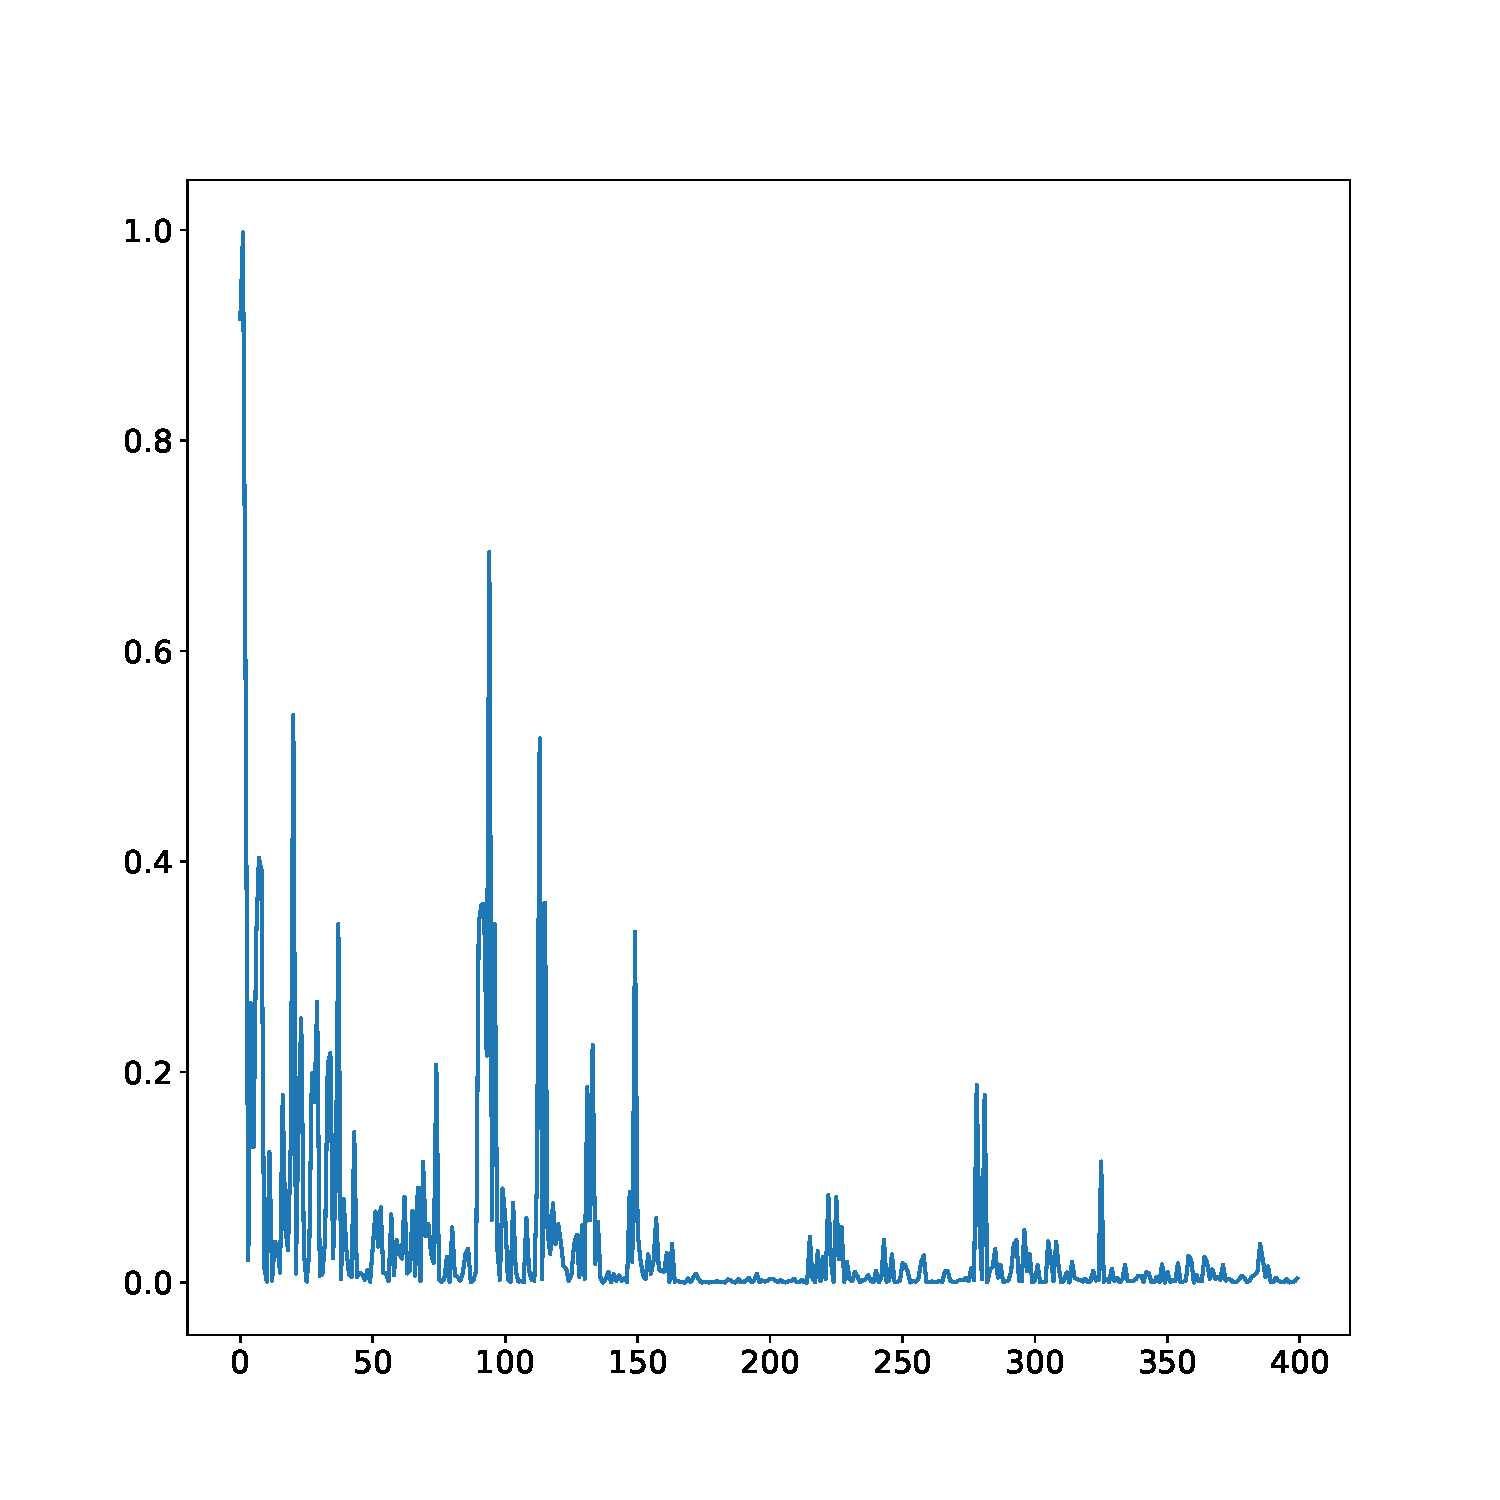
\includegraphics[width=\textwidth]{figure/cur.pdf}
			\caption{训练过程中输出误差变化图}\label{pic:误差变化图}
		\end{minipage}
		\begin{minipage}[t]{0.5\textwidth}
			\centering
			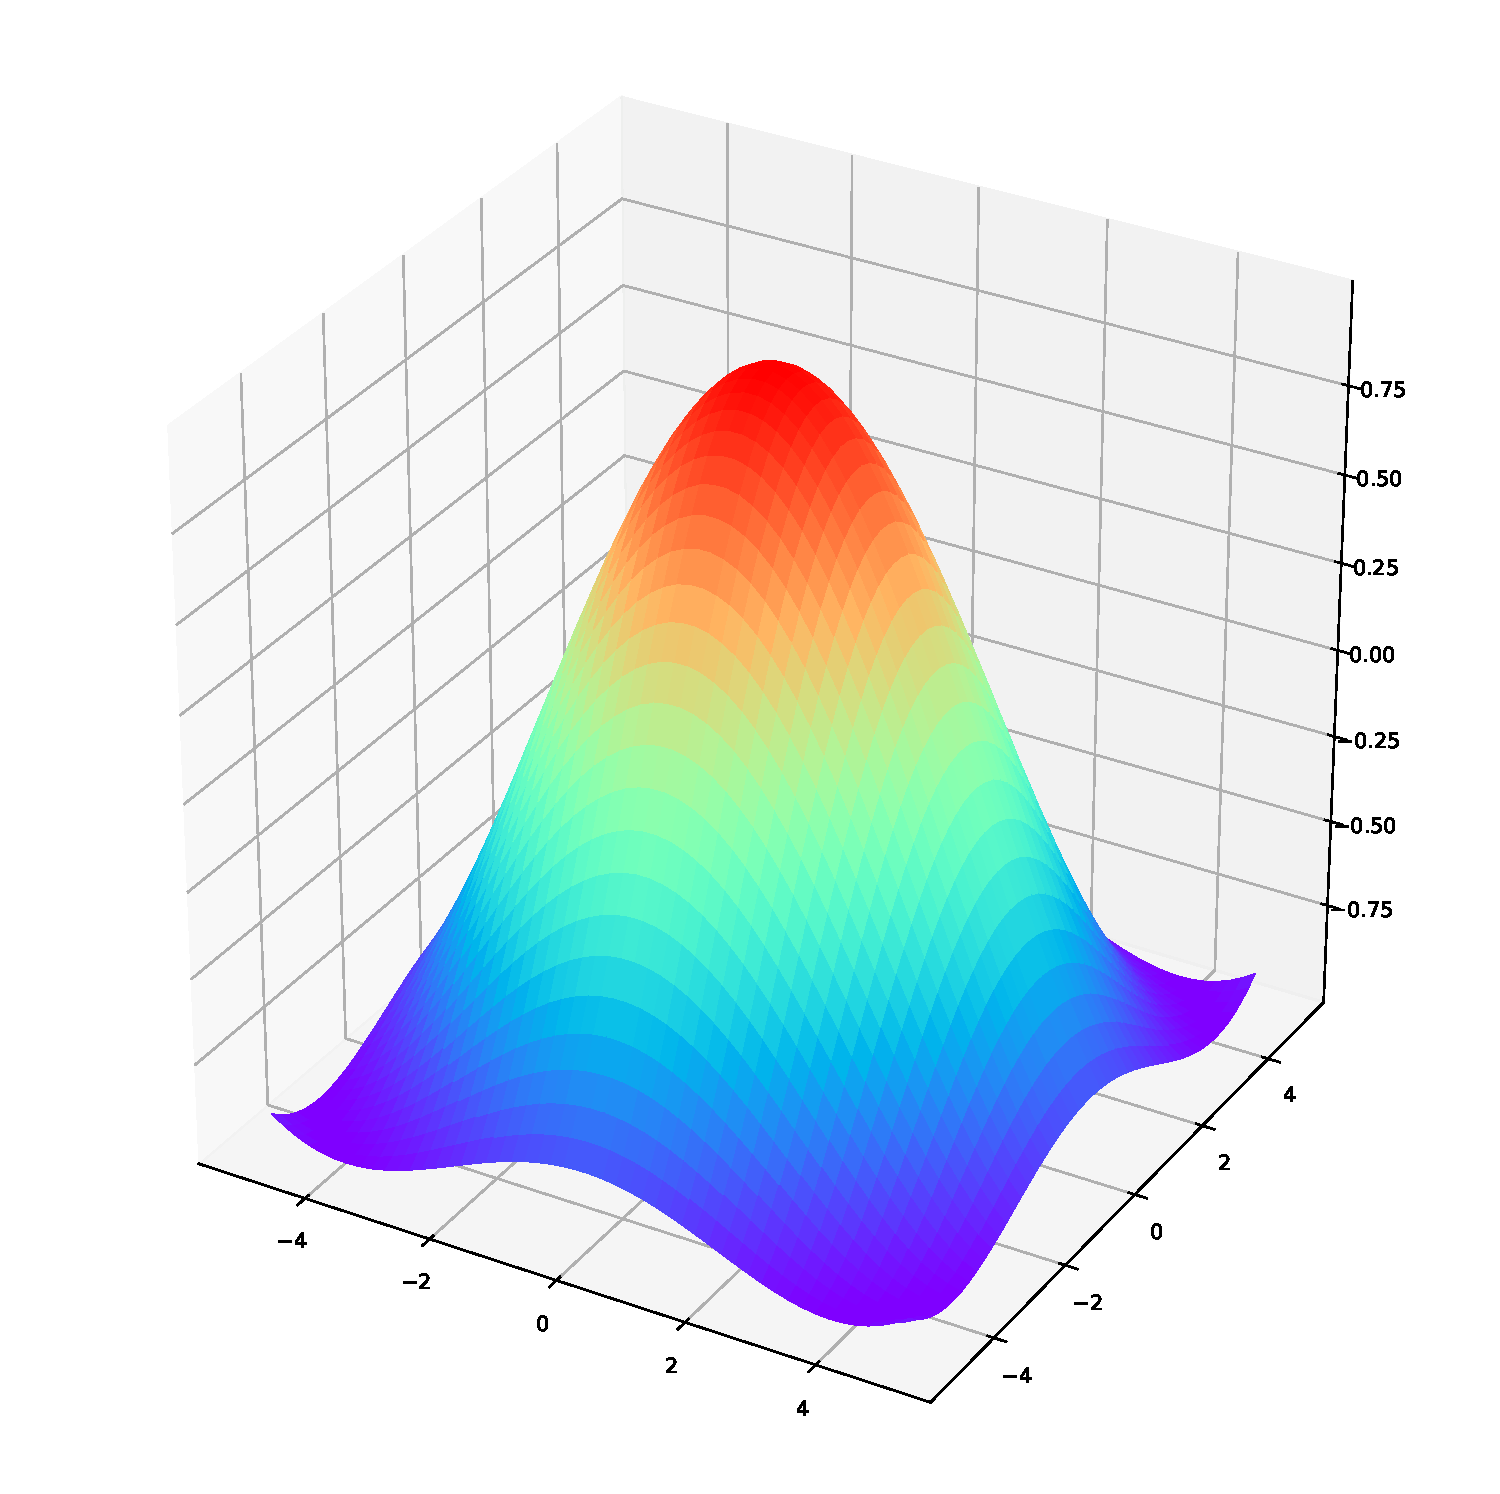
\includegraphics[width=\textwidth]{figure//target.pdf}
			\caption{期望的输入输出关系}\label{pic:期望关系图}
		\end{minipage}
	\end{figure}
	
	\section{正则化}
	正则化(Regularization)原本是用在线性回归中用于对不适定问题(ill-posed problem)进行回归的一种分析方法,后来被推广到人工智能领域,用于解决机器学习中的过拟合(over-fitting)问题\cite{RN132},即神经网络在训练集上表现很好而在测试集上表现较差的现象。正则化的基本思想是通过在训练中利用一些与过拟合有关的额外信息,对网络的过拟合进行抑制。在人工神经网络中使用的正则化方法主要有利用权值大小信息的L1正则化\cite{RN135}和L2正则化\cite{RN79}、利用神经元之间依赖性信息的Dropout\cite{RN133}、利用神经网络测试集表现的提前停止(early stopping)\cite{RN134}等。
	\subsection{L1正则化和L2正则化}
	L1正则化和L2正则化都是通过修改神经网络的损失函数实现对神经网络中过大的连接权值进行抑制,进而达到使神经网络正则化的目的。
	
	以\ref{sec:多层感知机}中的多层感知机为例,加入L1正则化和L2正则化操作后,神经网络的损失函数定义如下:
	\begin{equation}
		E_{Regularization}=E+R(\bm W)
	\end{equation}
	其中$E$为不加正则化时的网络损失函数,$R(\bm W)$为正则化项。在L1正则化时,$R(\bm W)$表达式为:
	\begin{equation}
		R(\bm W)=\sum_{i,j,l}|\omega_{ij}^{(l)}|
	\end{equation}
	即网络中所有神经元连接权值的绝对值之和。在L2正则化时,$R(\bm W)$表达式为:
	\begin{equation}
		R(\bm W)=\sum_{i,j,l}(\omega_{ij}^{(l)})^2
	\end{equation}
	即网络中所有神经元连接权值的平方之和。可以看出,不论是L1正则化还是L2正则化,基本的思想都是希望通过在损失函数中对过大的神经元连接权值添加“惩罚”项,减小使得神经网络的输入对输出的影响,进而使模型不能任意拟合训练数据中的随机噪声,从而达到减少过拟合的目的。

	\subsection{Dropout}
	Dropout方法最先由Hinton于2012年提出,是一种通过阻止一个较为复杂的前馈神经网络中有过多神经元的共同作用来防止神经网络过拟合的方法\cite{RN133}。Dropout可以作为训练深度神经网络的一种优化方法供选择。在每个训练批次中,通过忽略一定数量的神经元输出,可以明显地减少过拟合现象。这种方式可以减少隐藏层神经元间的依赖性(一个神经元需要靠其他神经元的激活才能发挥作用)。实际应用中,Dropout方法以Dropout层的形式存在于神经网络中,一个Dropout层由多个Dropout单元构成,有如下性质\cite{JMLR:v15:srivastava14a}:
	\begin{enumerate}[itemindent=2em,label=(\arabic*)]
		\item Dropout层的Dropout单元个数与上一层的神经元个数相同;
		\item 当前向传播算法计算到Dropout层时,Dropout单元的输出为(设Dropout层为第$l$层):
		\begin{equation}
			\begin{split}
				y_j^{(l)}&=y_j^{(l-1)}\frac{d_j^{(l)}}{p}\\
				d_j^{(l)}&=\left\{
					\begin{aligned}
						1&&(\mbox{概率为}p)\\
						0&&(\mbox{概率为}1-p)
					\end{aligned}
					\right.
			\end{split}
		\end{equation}
		其中,$d_j^{(l)}$为Dropout单元的清除标记,$p$为预先指定的Dropout层的失活概率。
		\item 当反向传播算法计算到Dropout层时,Dropout单元的误差信号为:
		\begin{equation}
			E_j^{(l)}=E_j^{(l-1)}\frac{d_j^{(l)}}{p}
		\end{equation}
		其中,清除标记$d_j^{(l)}$在上一次前向传播时确定。
	\end{enumerate}
	Dropout层的性质可以看出,Dropout层实际上是用于在训练阶段使前一层的神经元随机“失活”,“失活”的神经元在前向传播时输出为0,其余神经元的输出按设定失活概率的倒数增大,从而使得传递到下一层的输出总和与Dropout层时保持一致;反向传播时与失活神经元之间相连的神经元连接权值不进行更新(变化为0)。

	\subsection{提前停止}
	提前停止方法的基本假设是:一个会出现过拟合的神经网络,其过拟合程度随训练次数的增加而增加\cite{RN134}。在这个假设条件下,一定存在某一个时刻,神经网络在训练集上的表现和其过拟合的程度达到某种折中的状态,即网络训练得恰到好处,既有较好的性能,又没有出现很强的过拟合。提前停止的核心即是要在训练过程中找到这种恰到好处的状态,并停止训练,防止网络出现过拟合从而达到正则化的目的。

	神经网络的过拟合一般通过神经网络在训练集和测试集上的性能差异来评价,当神经网络在训练集上表现较好,但在测试集表现较差,说明神经网络已经出现了过拟合。按照这种方法,使用提前停止方法对神经网络进行训练的步骤如下:
	\begin{enumerate}[itemindent=2em,label=(\arabic*)]
		\item 将原始的训练数据集划分成训练集和测试集;
		\item 只在训练集上进行训练,并每隔一个固定周期计算模型在测试集上的误差;
		\item 当模型在测试集上的误差比上一次训练结果差的时候停止训练;
		\item 使用上一次迭代结果中的参数作为模型的最终参数。
	\end{enumerate}

	\section{卷积神经网络}
	卷积神经网络(Convolutional Neural Network,CNN)是对一般多层感知机的一种扩展,广泛应用于计算机视觉、自然语言处理等领域\cite{RN137}。在卷积神经网络中,除了输出部分的多层感知机(又称全连接层)还包含一个或多个卷积层(convolutional layer)、激活层(Rectified Linear Units layer,ReLU layer)和池化层(pooling layer)\cite{RN136}。
	\subsection{卷积层}
	卷积神经网络中每层卷积层由若干卷积核组成,每个卷积核的参数都对应一个权重系数和一个偏置,与人工神经元类似。卷积层内每个卷积核都与前一层中位置接近的区域的多个神经元输出相连,区域的大小取决于卷积核的大小,连接区域又称“感受野(receptive field)”,卷积核在工作时,会有规律地扫过输入特征,在感受野内对输入特征做矩阵元素乘法求和并叠加偏置,其表达式如下\cite{RN136}:
	\begin{equation}
		\begin{split}
			\bm Y^{(l+1)}\left(i,j\right)&=\left[\bm Y^{(l)}\otimes\bm\omega^{(l)}\right]\left(i,j\right)+\bm b\\
			&=\sum_{k=1}^{K_l}\sum_{x=1}^f\sum_{y=1}^f\left[\bm Y_{k}^{(l)}(s_0i+x,s_0j+y)\bm\omega_{k}^{(l+1)}(x,y)\right]+\bm{b}\\
			i,j&\in\left[0,L_{l+1}\right]\\
			L_{l+1}&=\frac{L_l+2p-f}{s_0}+1
		\end{split}
	\end{equation}
	其中$\bm b$为偏差量,$\bm Y^{(l)}$表示第$l$层的卷积输出,也被称为特征图(feature map),$L_{l+1}$为$\bm Y^{(l)}$的尺寸,$\bm Y^{(l)}(i,j)$对应特征图中的像素,$K_l$为特征图$\bm Y^{(l)}$的通道数,$f$、$s_0$和$p$分别对应卷积核大小、卷积步长(stride)和填充(padding)层数\cite{RN136}。一个典型的卷积核大小为3、卷积步长为1、填充层数为0的单通道二维卷积运算如图\ref{figure:二维卷积运算}所示。
	\begin{figure}[htbp]
		\centering
		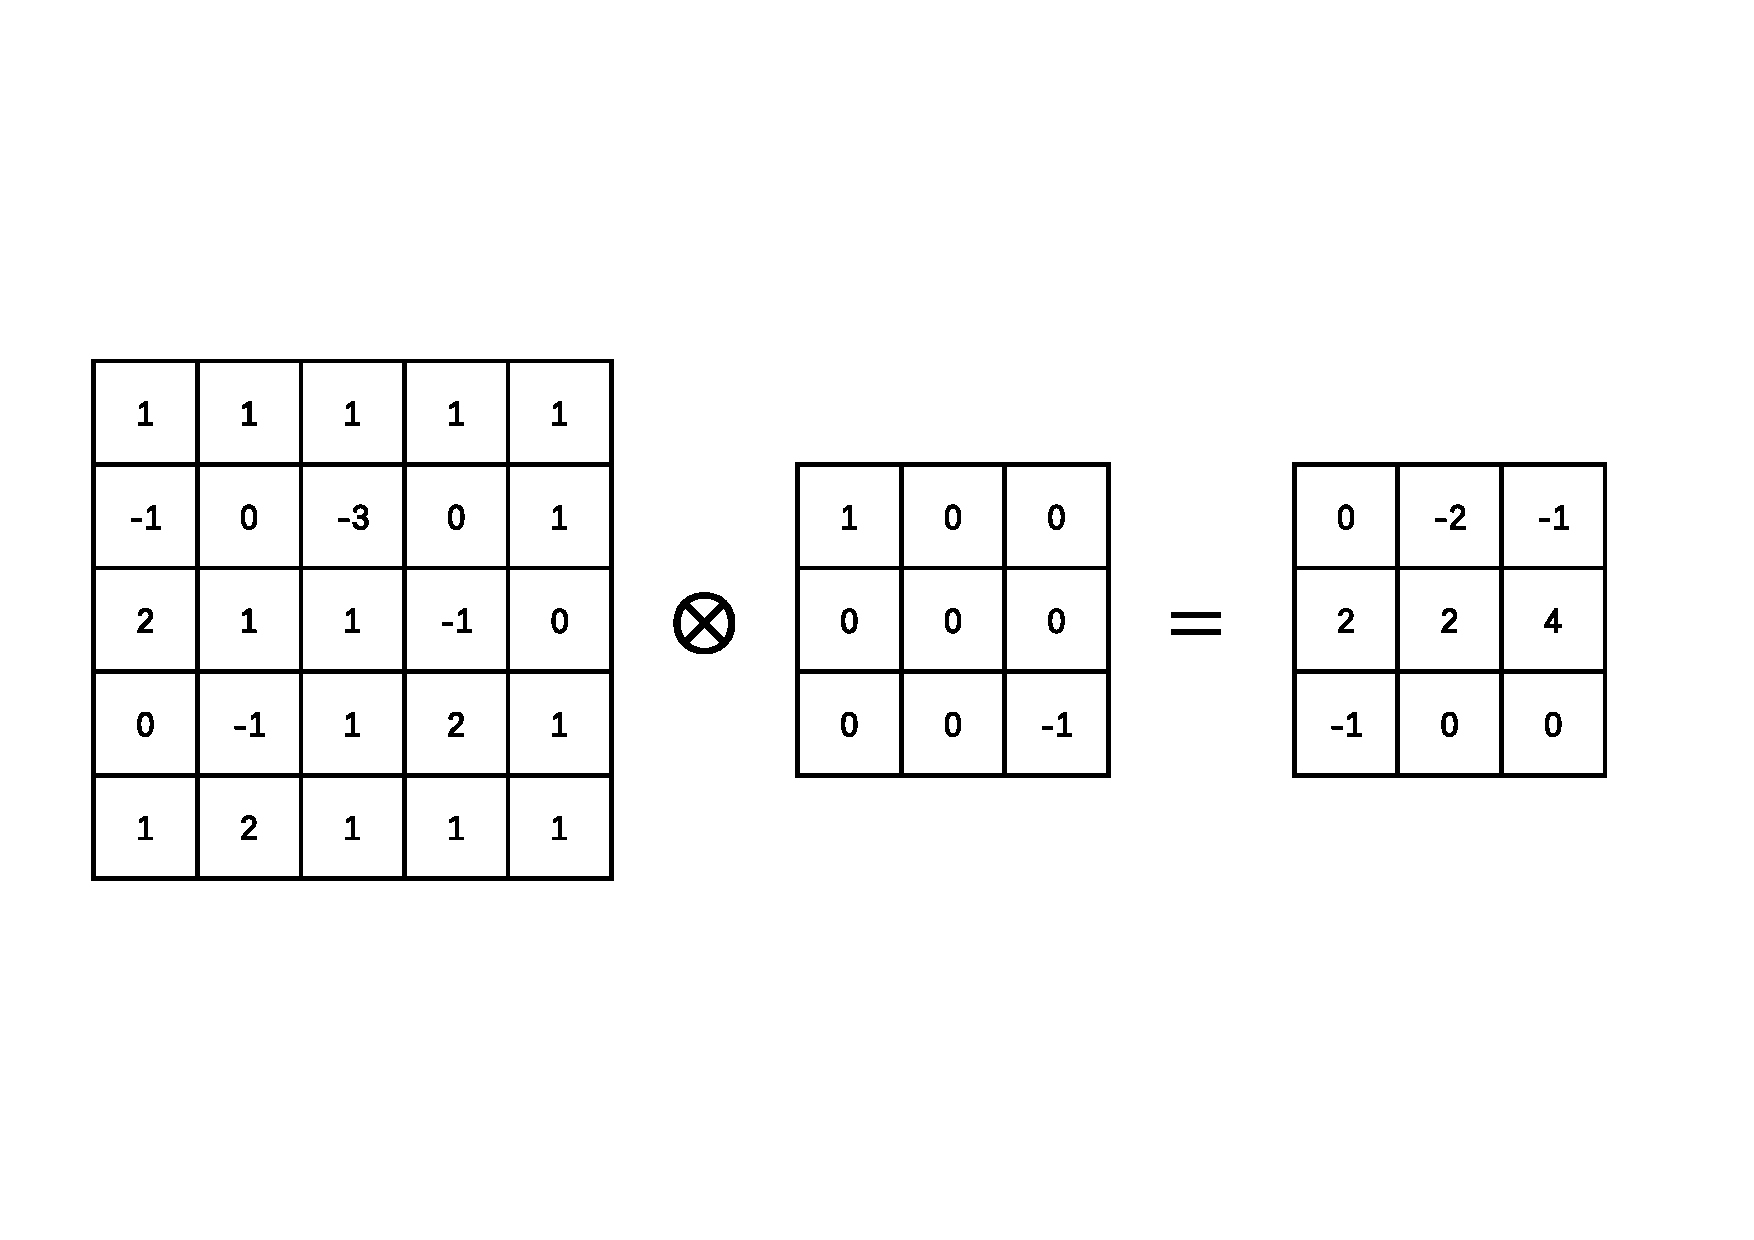
\includegraphics[width=0.9\textwidth, keepaspectratio]{figure/conv.pdf}\\
		\caption{二维卷积运算}\label{figure:二维卷积运算}
	\end{figure}

	卷积运算的目的是提取输入的不同特征,第一层卷积层可能只能提取一些低级的特征如边缘、线条和角等层级,更多层的网路能从低级特征中迭代提取更复杂的特征。
	
	\subsection{激活层}
	卷积神经网络的激活层和多层感知机的激活函数类似,都是将线性输入映射到非线性输出,以协助表达复杂特征。其表达式如下\cite{RN136}:
	\begin{equation}
		\bm Y^{(l)}(i,j)=f\left(\bm Y^{(l-1)}(i,j)\right)
	\end{equation}
	其中$f(\cdot)$为激活函数,通常采用ReLU函数及它的一些变体如有斜率的ReLU(Leaky ReLU, LReLU)、参数化的ReLU(Parametric ReLU, PReLU)、指数线性单元(Exponential Linear Unit, ELU)等。

	\subsection{池化层}
	在卷积层进行特征提取并经过激活层后,输出的特征图会被传递至池化层进行特征选择和信息过滤。卷积神经网络中一般采用最大值池化(max pooling),其表达式如下:
	\begin{equation}
		\bm Y^{(l)}\left(i,j\right)=max_{x=1\rightarrow f,y=1\rightarrow f}\left[\bm Y_{k}^{(l-1)}(s_0i+x,s_0j+y)\right]
	\end{equation}
	一个典型的$2\times 2$最大值池化操作如图\ref{figure:最大值池化操作}所示。
	\begin{figure}[htbp]
		\centering
		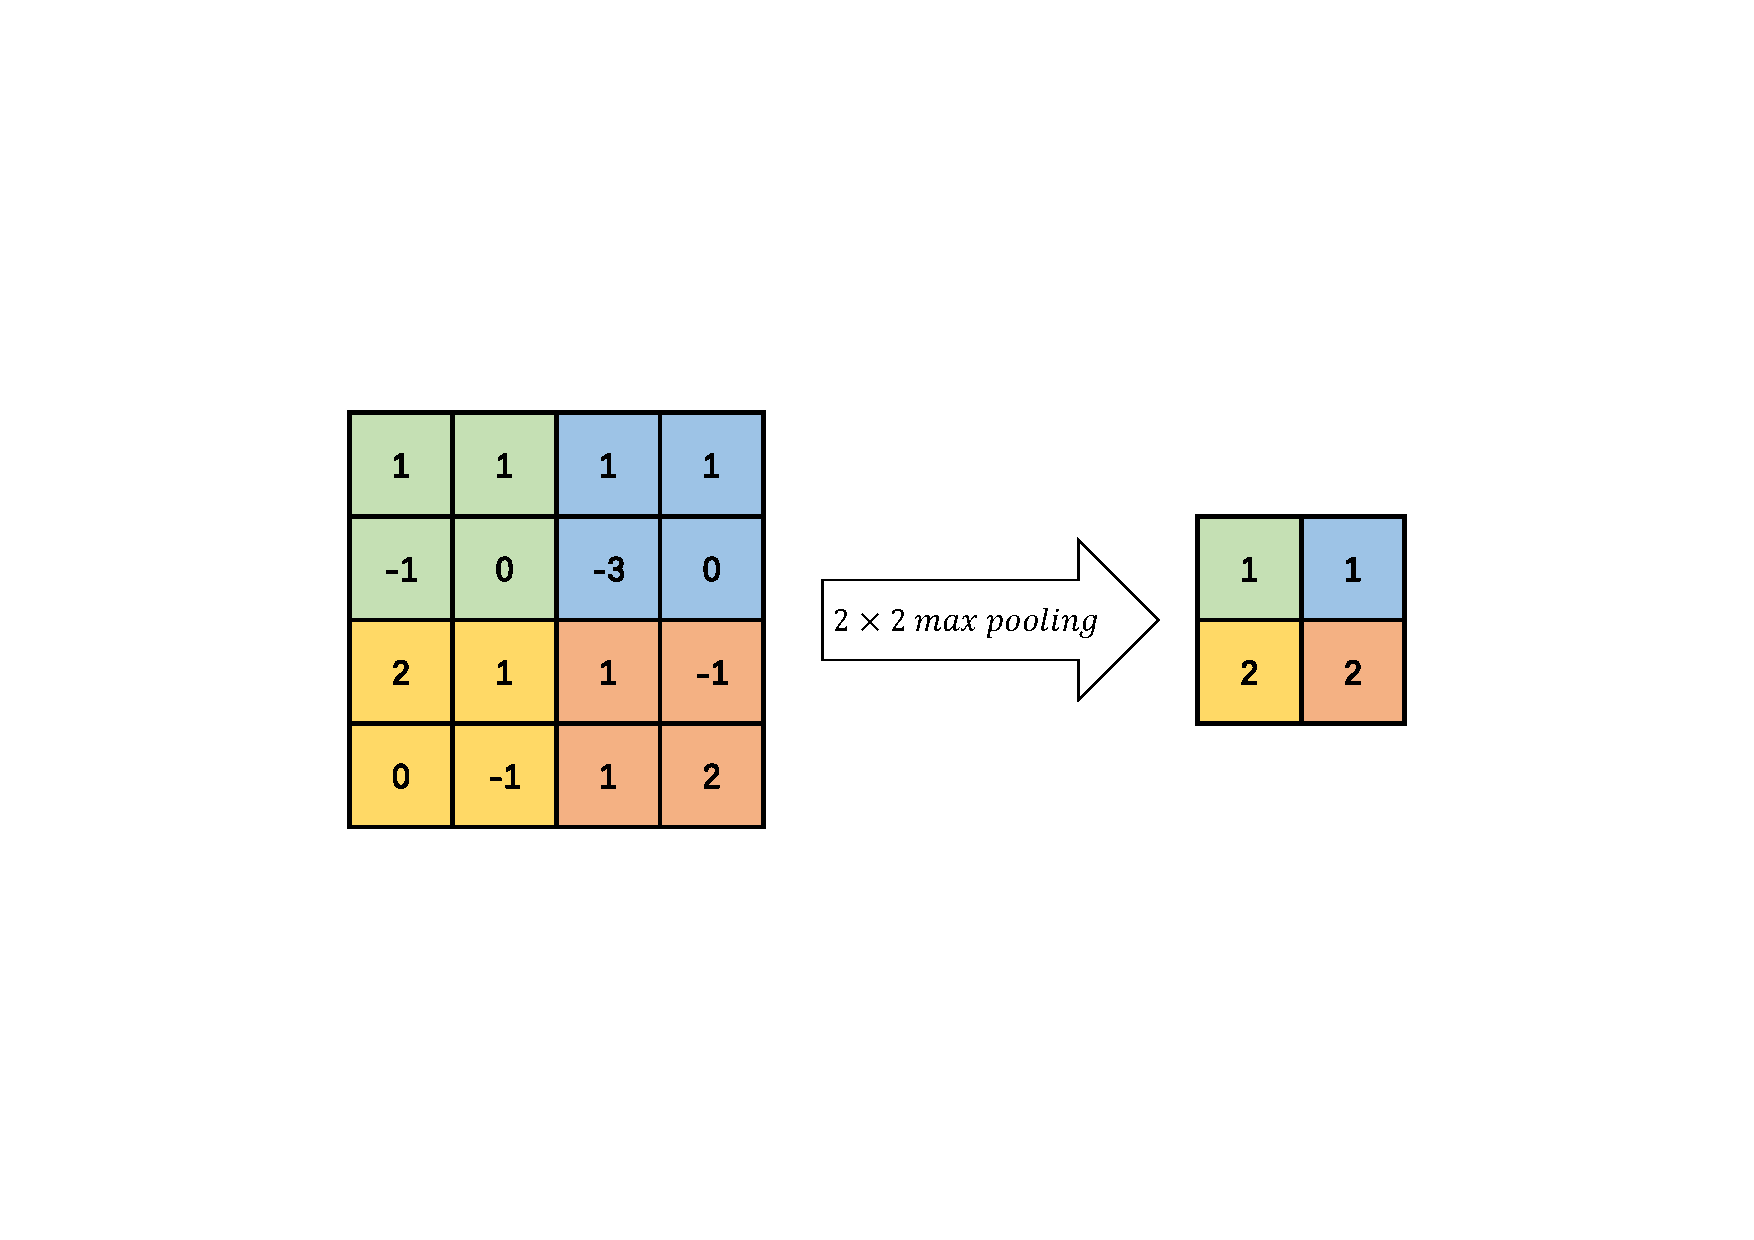
\includegraphics[width=0.8\textwidth, keepaspectratio]{figure/pooling.pdf}\\
		\caption{最大值池化操作}\label{figure:最大值池化操作}
	\end{figure}

\section{人工神经网络应用实例}
MNIST是来自美国国家标准与技术研究所(National Institute of Standards and Technology,NIST)的一个手写数字识别库,是世界上最权威的数字手写体数据库;CIFAR-10是由Hinton的学生Alex Krizhevsky和Ilya Sutskever整理的一个用于识别普适物体的小型数据集。这两个数据集是人工智能领域常用的基准测试。本文将以MNIST和CIFAR-10为例,结合前文所述的各类人工神经网络相关技术构建一个简单的图像识别模型,并对其进行评价。

\subsection{构建数据集}
MNIST数据集中包含70000个28$\times$28大小的数字手写体灰度图像,这些数据已经预先分为两个部分:包含60000个样本的训练集和包含10000个样本的测试集。CIFAR-10数据集中包含6个样本集共计60000张32$\times$32大小的3通道彩色图像,共有10个类别:飞机(airplane)、汽车(automobile)、鸟类(bird)、猫(cat)、鹿(deer)、狗(dog)、蛙类(frog)、马(horse)、船(ship)和卡车(truck)。6个样本集中5个用作训练集,一个作为测试集。训练集用于训练神经网络,测试集用于对训练完成的神经网络进行测试。

\subsection{构建模型}
手写体识别模型和CIFAR-10识别模型都基于经典的LeNet网络\cite{RN138},其结构如图\ref{figure:LeNet}所示。模型包含一个边长为5,输出通道数为20的卷积层、一个边长为5,输出通道数为50的卷积层、两个激活层、两个$2\times 2$池化层、一个隐藏层神经元数目为50的全连接层和一个Softmax层。其中全连接层和激活层所使用的激活函数为ReLU函数。手写体识别模型和CIFAR-10识别模型不同点在于,前者输入通道数为1,后者输入通道数为3。
\begin{figure}[htbp]
	\centering
	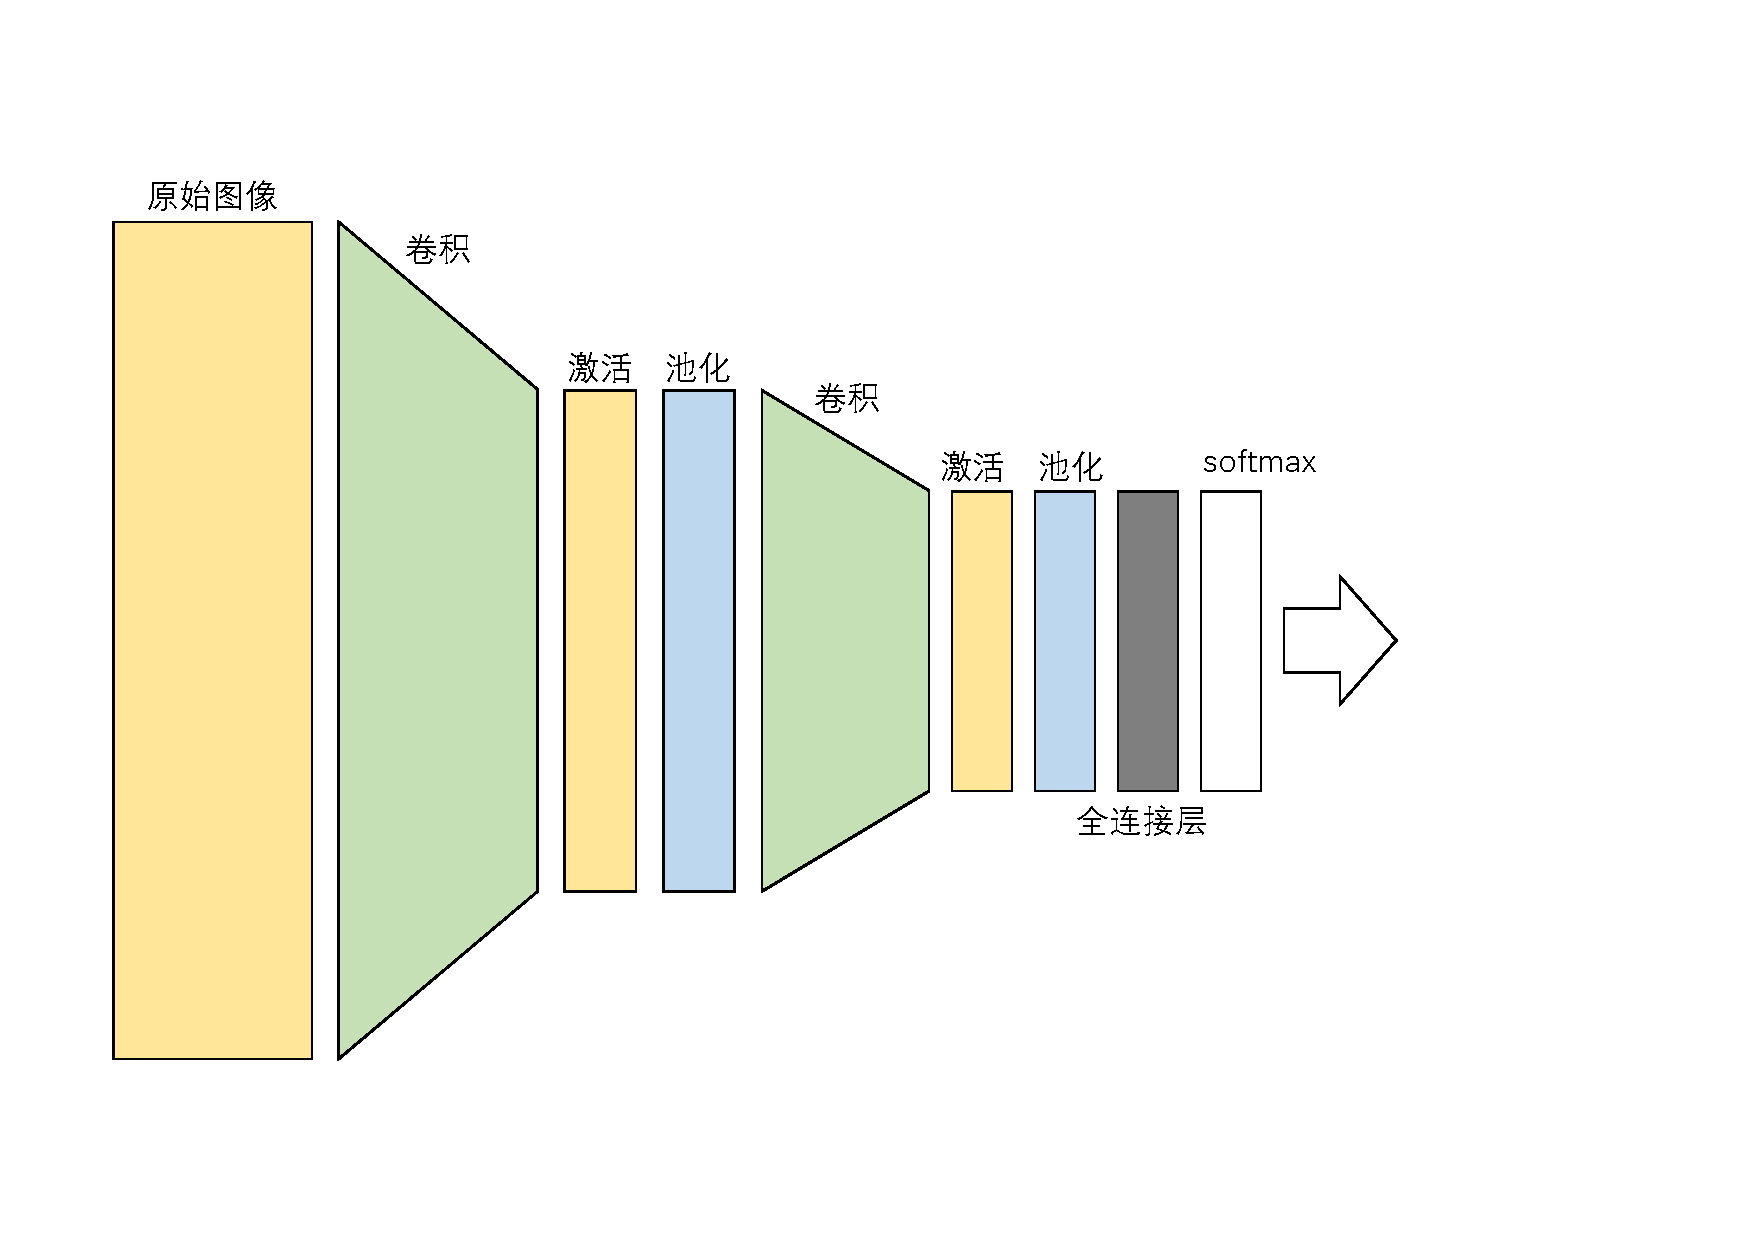
\includegraphics[width=0.8\textwidth, keepaspectratio]{figure/LeNet.pdf}\\
	\caption{LeNet网络结构}\label{figure:LeNet}
\end{figure}

\subsection{测试模型}
\subsubsection{基本模型测试}\label{sec:基本测试}
\begin{enumerate}[itemindent=2em,label=(\arabic*)]
	\item 使用MNIST训练集中的全部60000个样本进行训练,使用测试集中的全部10000个样本对模型进行测试。训练-测试的过程重复10次可以得到LeNet在MNIST测试集上的平均正确率为98.279\%。
	\item 使用CIFAR-10训练集中的全部50000个样本进行训练,使用测试集中的全部10000个样本对模型进行测试。训练-测试的过程重复10次可以得到LeNet在MNIST测试集上的平均正确率为61\%。
\end{enumerate}


\subsubsection{增加全连接层神经元数量}\label{sec:增加神经元数量}
将隐藏层神经元个数增加到200,训练方案和测试方案同\ref{sec:基本测试},可以得到LeNet在MNIST测试集上的平均正确率为98.566\%,在CIFAR-10测试集上的平均正确率为69\%。

\subsubsection{添加Dropout层}\label{sec:添加Dropout层}
在\ref{sec:增加神经元数量}的基础上,在网络全连接层输出添加一个$p=0.5$的Dropout层,训练方案和测试方案同\ref{sec:基本测试},可以得到LeNet在MNIST测试集上的平均正确率为98.566\%,在CIFAR-10测试集上的平均正确率为63\%。

\subsection{结果分析}
\ref{sec:增加神经元数量}中的结果印证了\ref{sec:多层感知机}中增加隐藏层神经元数量能提高神经网络拟合精度的结论,但也证明在数据集较为简单时,增加隐藏层神经元数量对神经网络精度的提升不明显,而在较为复杂的CIFAR-10数据集上,增加3倍的隐藏层神经元个数能将网络的性能提升提升约10\%;\ref{sec:添加Dropout层}中的结果表明,隐藏层神经元数量为200时,LeNet模型在较为简单的MNIST数据集训练的过程中存在一定的过拟合,通过添加Dropout层能进一步提高LeNet模型在MNIST测试集上的精度。但是在更为复杂的CIFAR-10数据集上,LeNet模型中由200个神经元组成的隐藏层并不足以产生明显的过拟合现象,添加Dropout层反而会影响网络的训练效果,降低模型的测试精度。

\section{总结}
在人工神经网络提出至今的半个多世纪里,对于人工神经网络理论和应用的研究取得了长足的发展。神经元模型的多样化、神经网络结构的多样化、训练方式的多样化、以及突破分层的神经网络模型开发新的网络结构,是目前人工神经网络研究的突出发展方向。近年来,各类新兴神经元模型和神经网络模型的发展有效促进了回归分析技术的提升,例如递归神经网络(Recursive neural network)\cite{RN139},循环神经网络(Recurrent Neural Network,RNN)\cite{RN140}、编码解码模型(Encoder-Decoder model)\cite{RN143}、长短时记忆网络(Long Short-Term Memory,LSTM)\cite{RN141}、残差网络(ResNet)\cite{RN142}、生成对抗网络(Generative Adversarial Networks,GAN)\cite{RN144}等;与神经网络相关的各种训练与优化算法也在蓬勃发展,例如注意力(Attention)机制\cite{RN145}、Boosting方法\cite{RN146}、各种改进的梯度下降法\cite{RN147}\cite{RN148}\cite{RN149}等。人工神经网络及其相关领域的研究进展使人工智能在越来越多的场景中表现出超越人类的能力,也使得与人工神经网络和相关的训练与优化技术成为目前人工智能领域最受关注的发展方向。

本文对人工神经网络的基本思想方法进行了综述研究,并将人工神经网络相关的一些常见技术进行了归类介绍,并适当描述了各类方法之间、同类方法之间的一些差别与联系。本文还详细分析了各类方法的部分理论细节,给出了一个简单的应用示例,最后分析了人工神经网络的主要发展趋势。希望本文能对相关科研人员了解人工神经网络并开展相关研究起到微薄的作用。

\end{spacing}
\bibliography{ref}
\bibliographystyle{unsrt}
\end{document}